\thispagestyle{toancuabinone}
\pagestyle{toancuabi}
\everymath{\color{toancuabi}}
%\blfootnote{$^1$\color{toancuabi}Đại học Thăng Long.}
\graphicspath{{../toancuabi/pic/}}
\begingroup
\AddToShipoutPicture*{\put(0,616){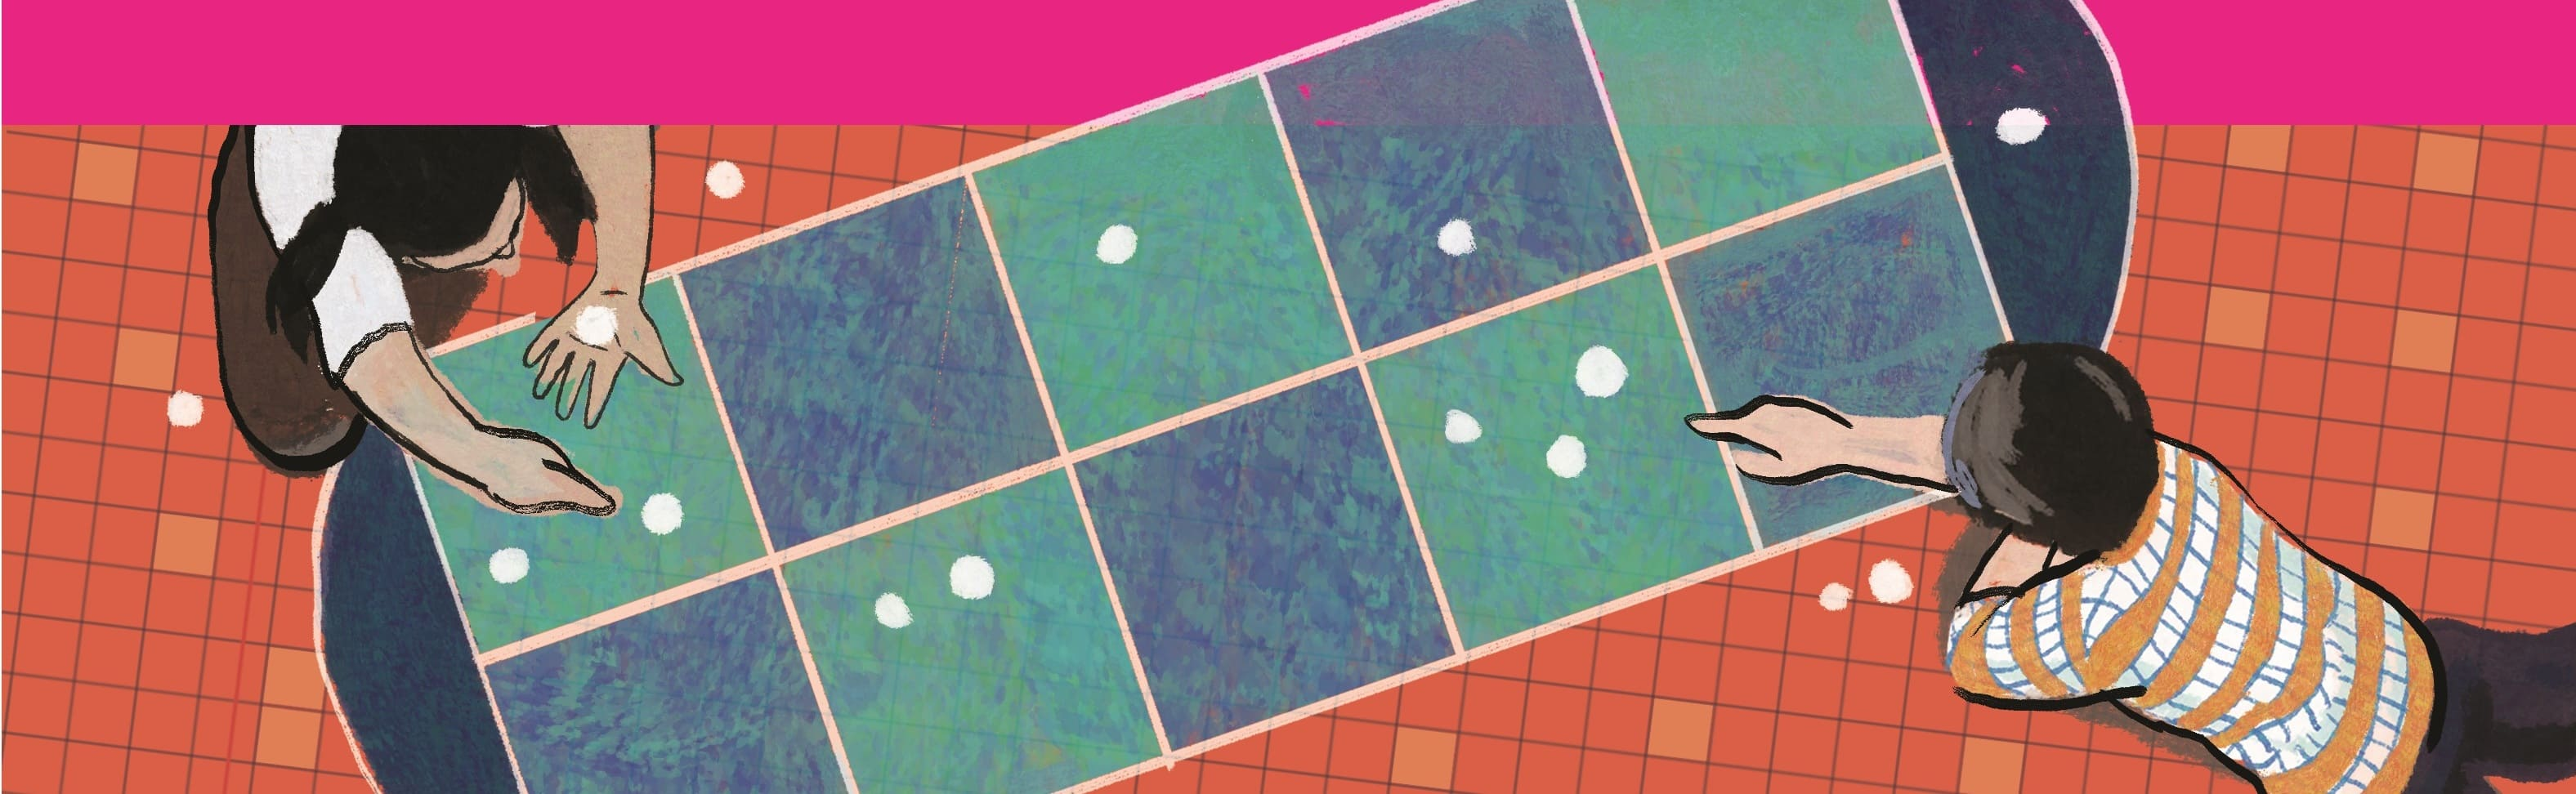
\includegraphics[width=19.3cm]{../bannertoancuabi}}}  
\AddToShipoutPicture*{\put(78,550){
\includegraphics[scale=1]{../tieude.pdf}}} 
\centering
\endgroup
\vspace*{160pt}

\begin{multicols}{2}
	Để điều tra một vụ án về kinh tế, Thám tử Xuân Phong cần thẩm vấn các đại diện của hai công ty vốn cạnh tranh kịch liệt với nhau là Sungsang và TungTeng. Qua thư ký bố trí xếp lịch, Xuân Phong mời được ba người là ông Kim, ông Lee và ông Han của hai công ty đình đám nọ tới văn phòng. Lịch sử cạnh tranh hàng chục năm nay của hai công ty này luôn chỉ ra rằng: các đại diện của cùng một công ty luôn nói thật với nhau, còn với đại diện của công ty cạnh tranh lại luôn \linebreak nói dối. 
	\vskip 0.1cm
	Các vị khách có mặt đúng giờ tại văn phòng thám tử  trong các bộ com--lê sang trọng xứng với đẳng cấp của đại diện cho các công ty hàng đầu về công nghệ. Vừa nhìn thấy  nhau, ông Kim đã  tiến tới trước mặt ông Lee và nói ``Tôi tới từ công ty Sungsang". Ông Lee trả lời ngay ``Ô thế à! Vậy là ông và ông Han cùng làm ở một công ty đấy!".
	\vskip 0.1cm
	Từ đoạn hội thoại trên, Xuân Phong xác định được ngay ông Han làm ở công ty nào. Em có thể lập luận xem làm cách nào mà thám tử lại biết vậy được không?
\end{multicols}
\begin{figure}[H]
	\centering
	\vspace*{-5pt}
	\captionsetup{labelformat= empty, justification=centering}
	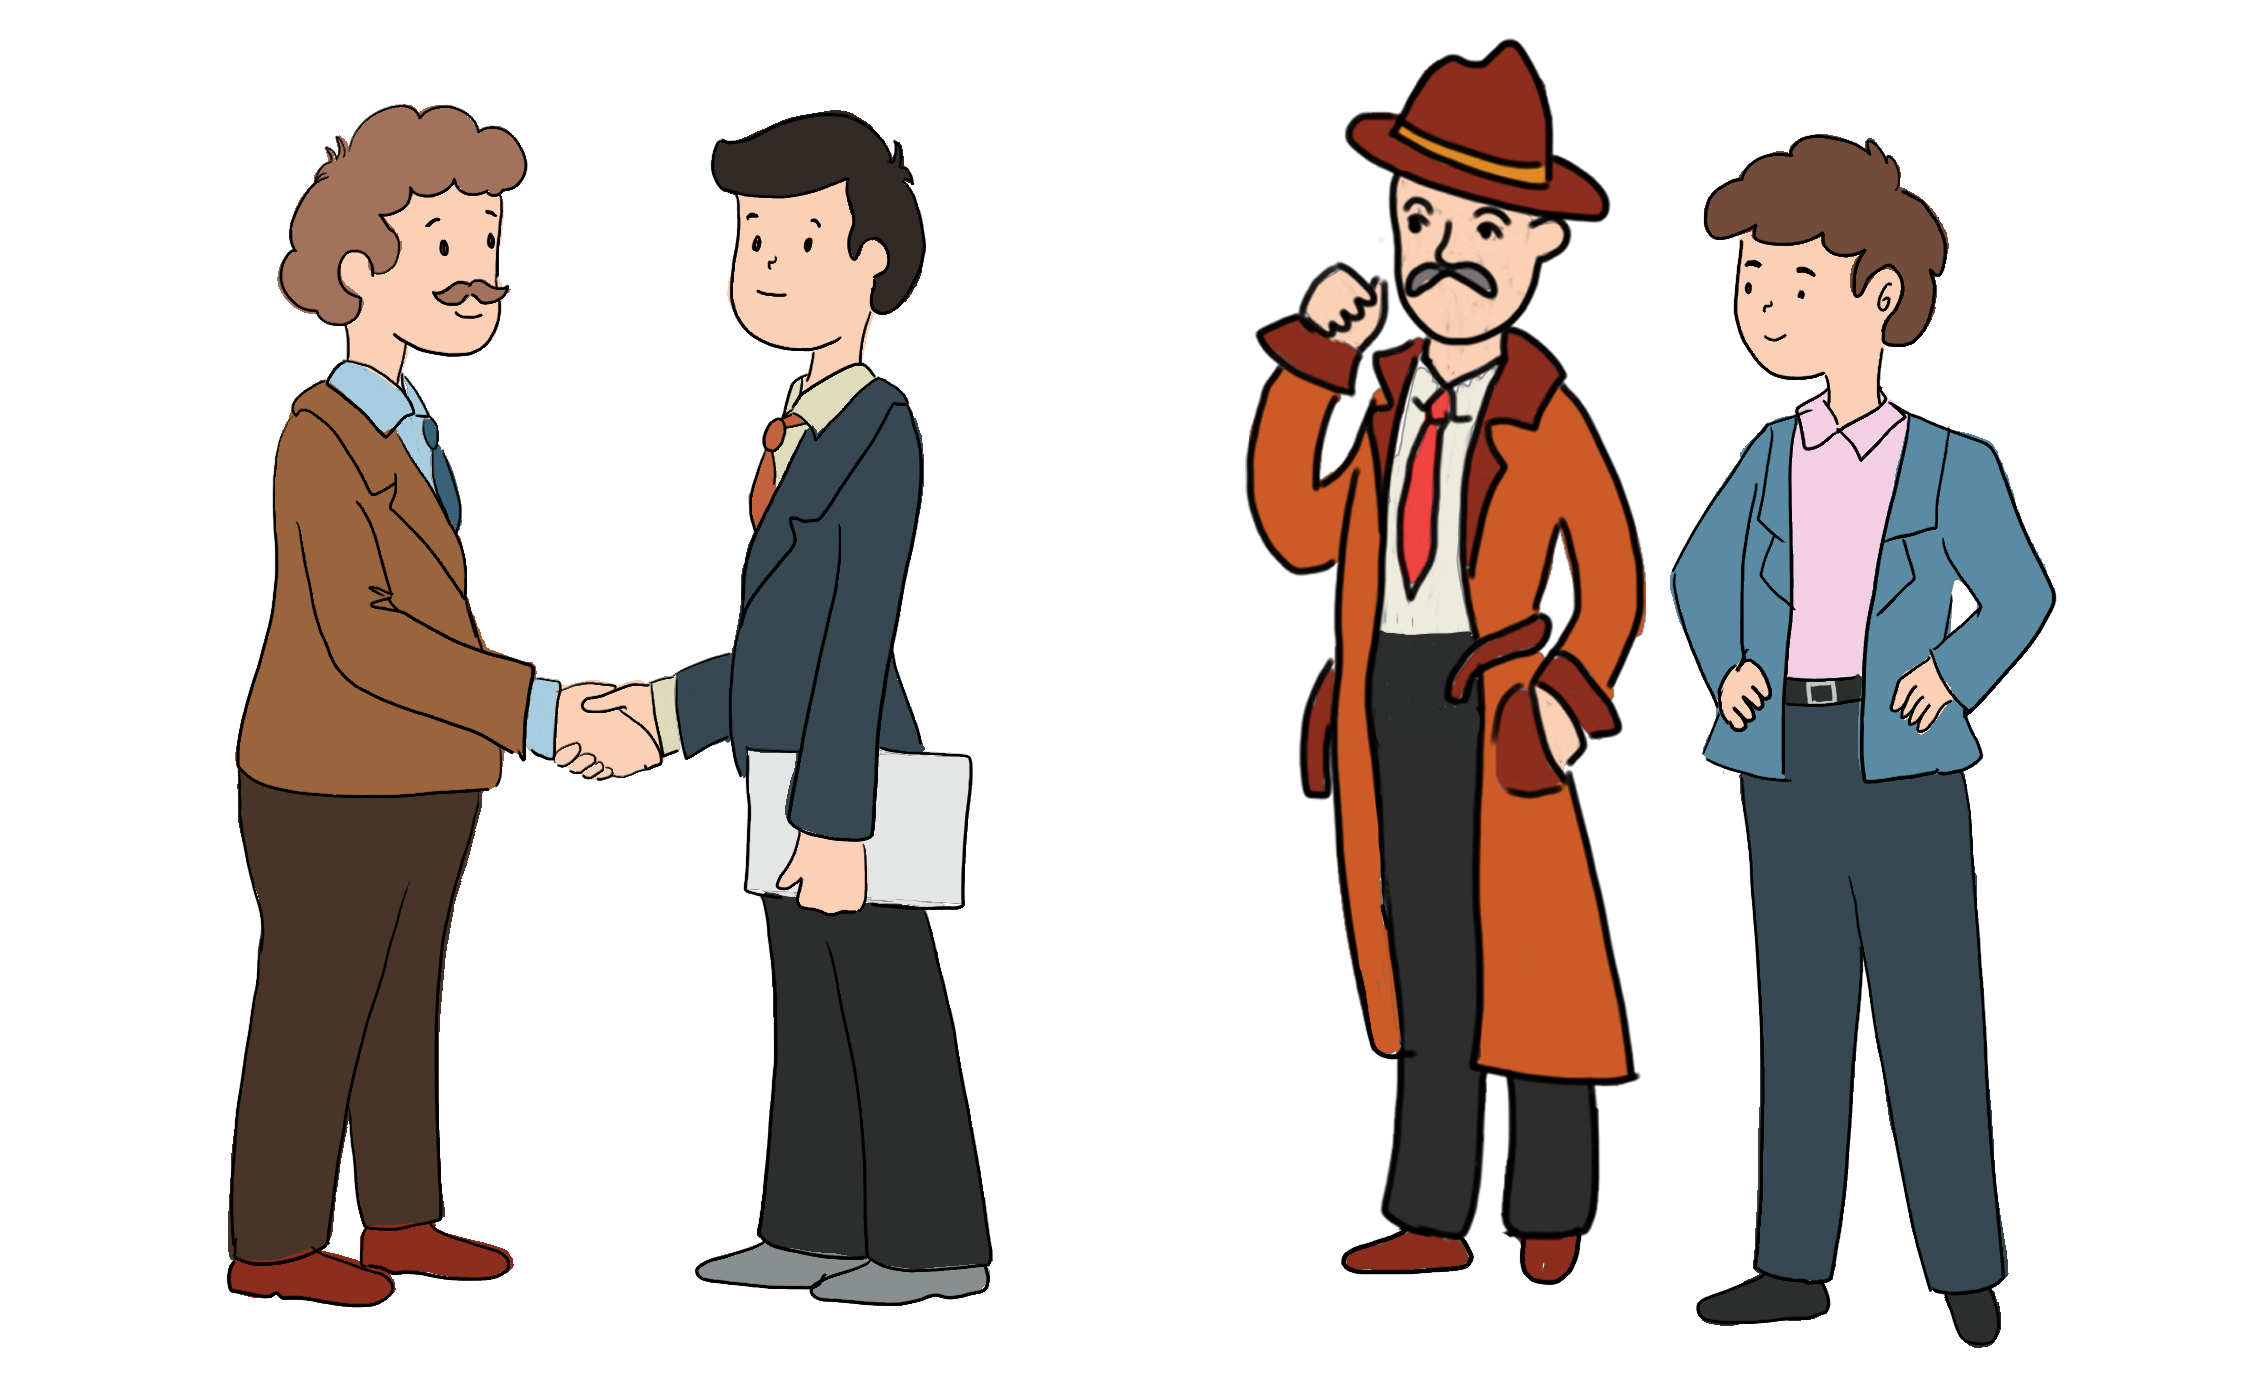
\includegraphics[width=1\linewidth]{xuanphong}
	\vspace*{-5pt}
\end{figure}
\newpage
\begingroup
\AddToShipoutPicture*{\put(115,670){
\includegraphics[scale=1]{../tieude11.pdf}}} 
\centering
\endgroup
\vspace*{33pt}

\begin{multicols}{2}
	$\pmb{1.}$	Bạn Công đã trả $24$ nghìn đồng để mua được $1$ cuốn vở, $2$ chiếc bút chì và $1$ cái tẩy. Bạn Nam thì trả tận $54$ nghìn đồng để mua được $2$ cuốn vở, $3$ chiếc bút chì và $3$ cái tẩy. Hỏi bạn An đã trả bao nhiêu tiền để mua được $2$ cuốn vở, $5$ chiếc bút chì và $1$ cái tẩy?
	\begin{figure}[H]
		\centering
		\vspace*{-5pt}
		\captionsetup{labelformat= empty, justification=centering}
		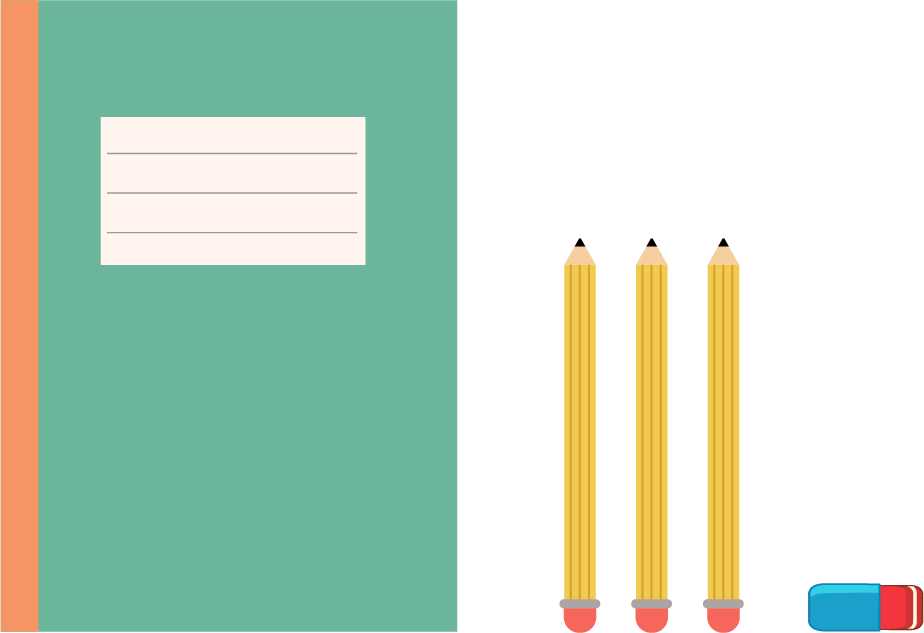
\includegraphics[width=1\linewidth]{Pi3_bai1}
		\vspace*{-10pt}
	\end{figure}
	$\pmb{2.}$ Bác Tuyết mang sữa đựng đầy trong hai chiếc thùng ra chợ bán. Lượng sữa trong thùng to nhiều gấp $3$ lần lượng sữa trong chiếc thùng nhỏ. Khi trong chiếc thùng nhỏ còn có $15$ lít sữa, còn thùng to còn $35$ lít sữa, bác Tuyết đổ dồn một lượng sữa từ thùng to cho đầy chiếc thùng nhỏ. Khi đó trong chiếc thùng to lượng sữa còn lại  đầy tới một nửa thùng. Hỏi bác Tuyết đã đổ bao nhiêu sữa từ thùng to sang thùng nhỏ, và dung tích của mỗi thùng là bao nhiêu?
	\begin{figure}[H]
		\centering
		\vspace*{-10pt}
		\captionsetup{labelformat= empty, justification=centering}
		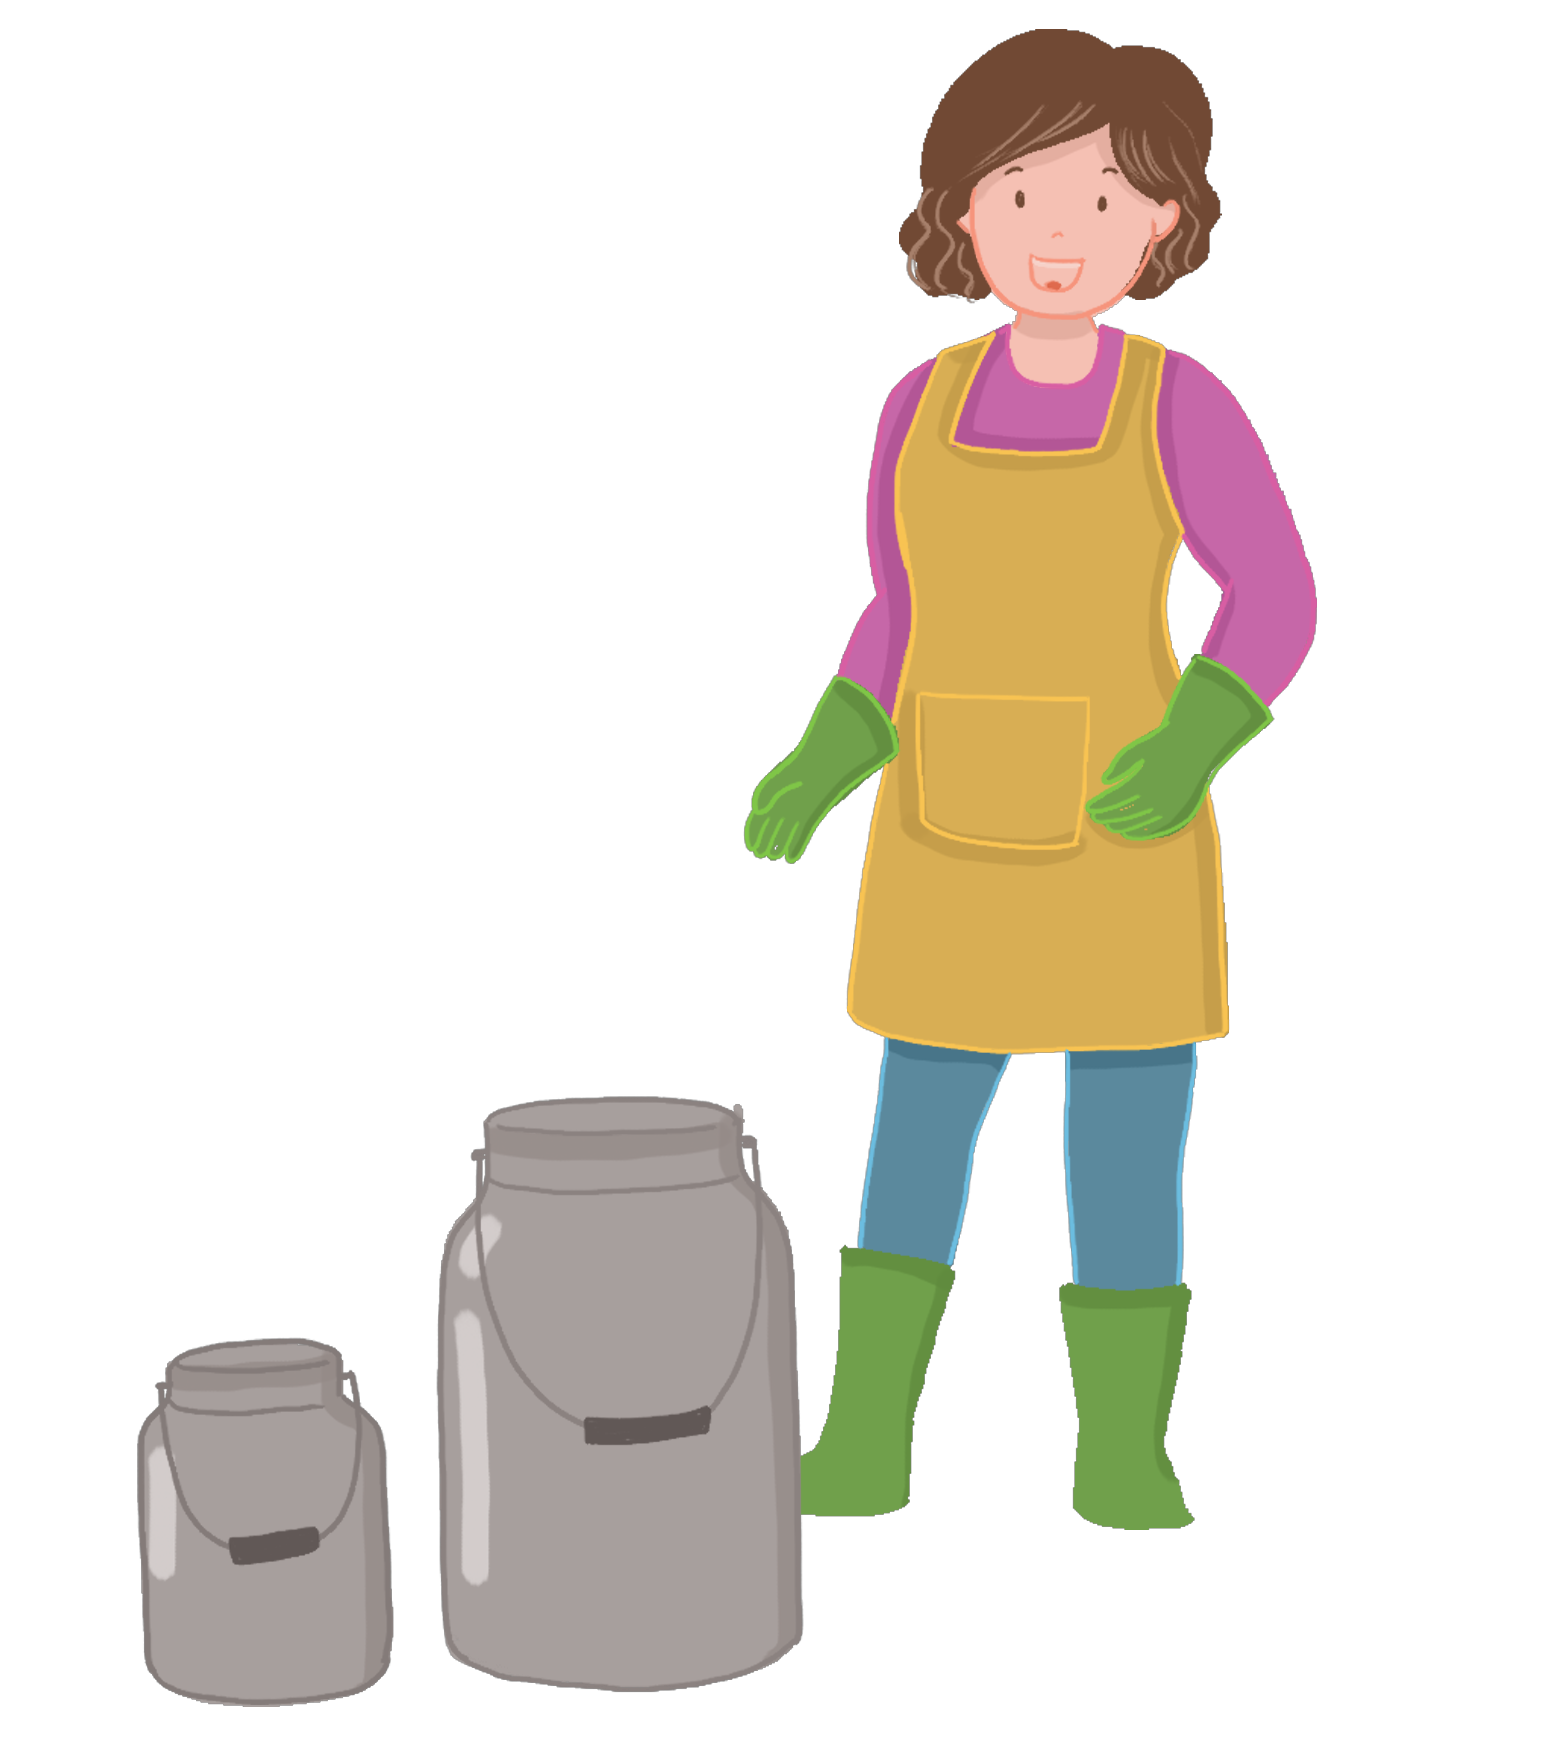
\includegraphics[width=0.75\linewidth]{Pi3_bai2}
		\vspace*{-5pt}
	\end{figure}
	$\pmb{3.}$ Một tấn hoa quả được chở tới siêu thị: táo được đóng theo các thùng gỗ  $48$ kg/thùng, lê được đóng trong các thùng gỗ $20$ kg/thùng, mận đựng trong hộp giấy theo $14$ kg/hộp còn nho đựng trong các hộp giấy theo $10$ kg/hộp. Biết rằng số kg táo được chở tới nhiều gấp đôi số kg lê, còn số kg mận và nho là bằng nhau, hỏi số lượng mỗi loại hoa quả đã được vận chuyển tới cửa hàng là bao nhiêu?
	\begin{figure}[H]
		\centering
		\vspace*{-5pt}
		\captionsetup{labelformat= empty, justification=centering}
		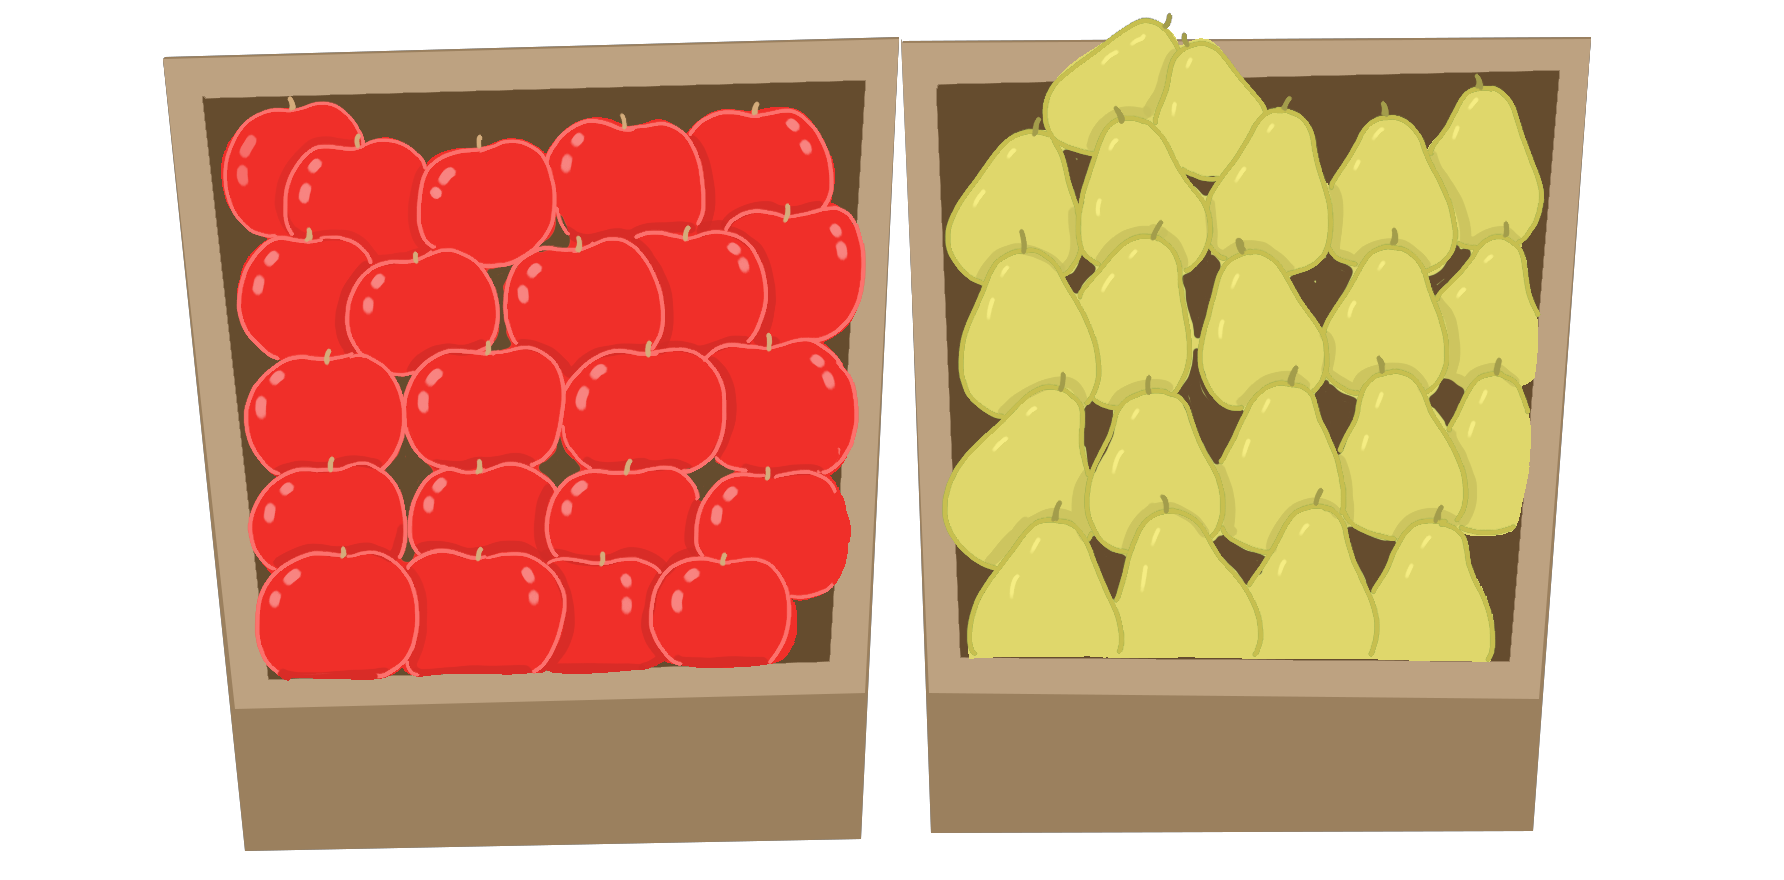
\includegraphics[width=1\linewidth]{Pi3_bai3}
		\vspace*{-10pt}
	\end{figure}
	$\pmb{4.}$ Bạn An khởi hành đi bộ từ làng $A$ tới làng $B$ lúc $8$h sáng. Đồng thời vào lúc đó, bạn Bình cũng đi bộ từ làng $B$ tới làng $A$. Hai bạn đều đi với vận tốc không đổi, nhưng có thể không bằng nhau. Khi gặp nhau ở giữa đường, bạn An còn phải đi thêm $32$ phút nữa, còn Bình phải đi thêm $18$ phút nữa thì mới tới nơi. Hỏi hai bạn đã gặp nhau sau bao lâu tính từ lúc khởi hành?
	\begin{figure}[H]
		\centering
		\vspace*{-5pt}
		\captionsetup{labelformat= empty, justification=centering}
		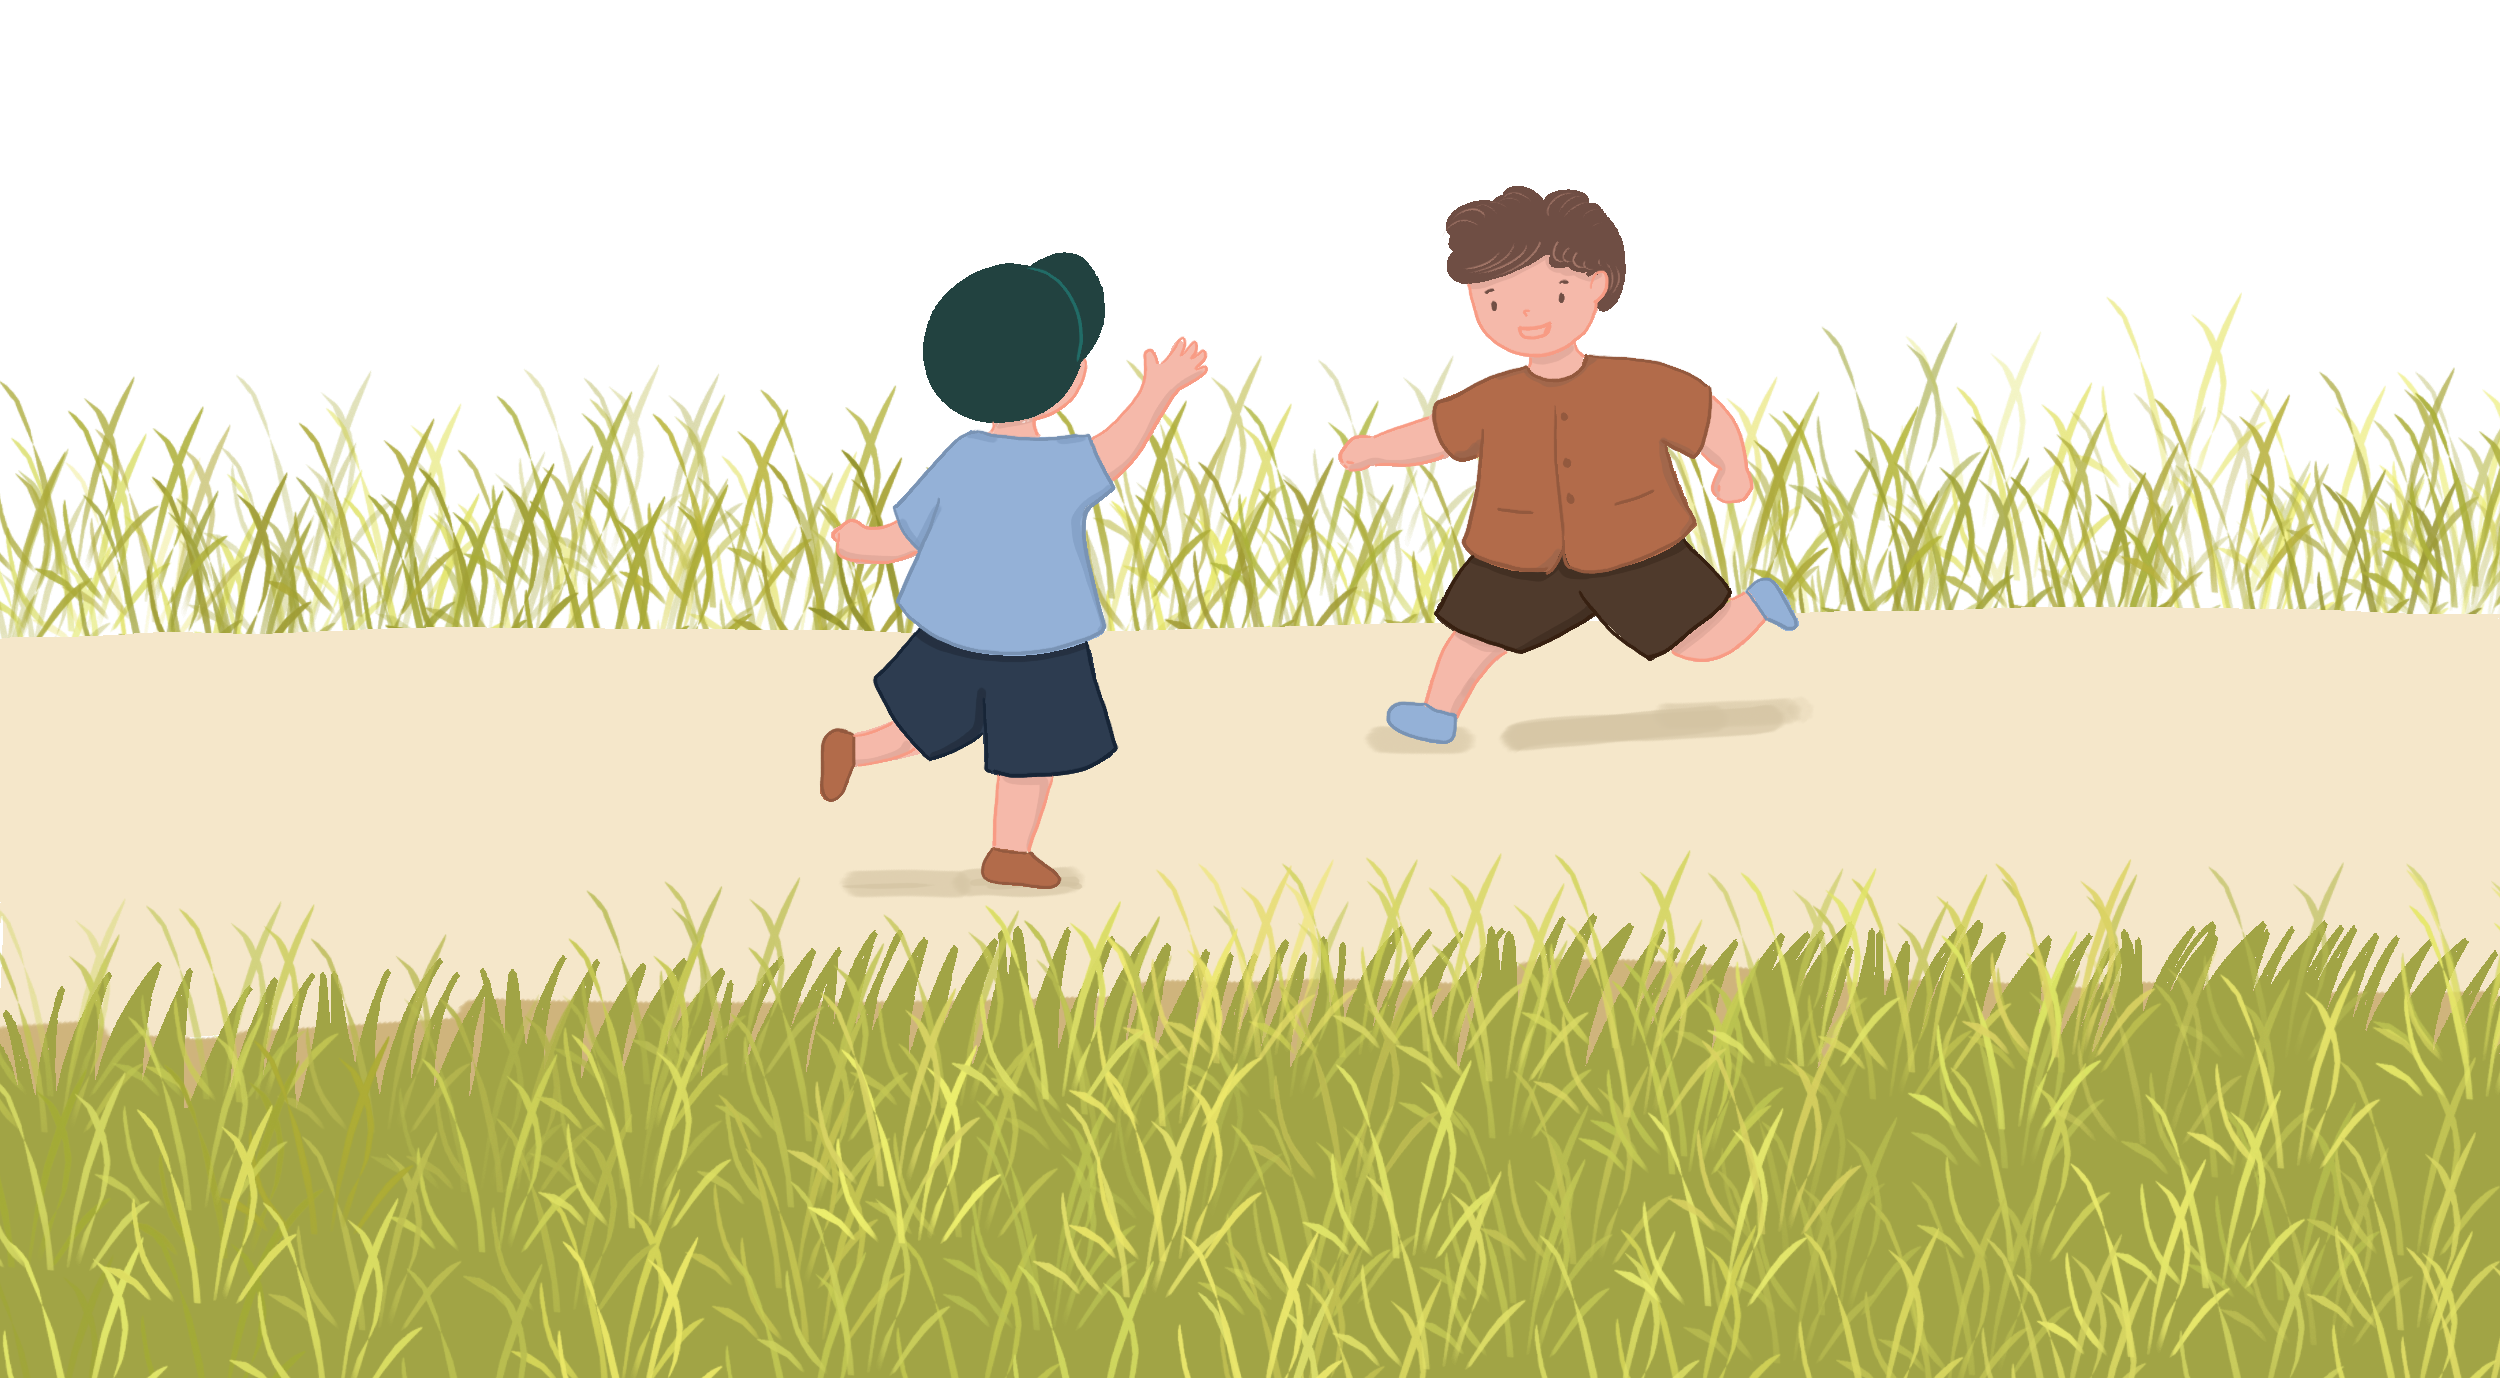
\includegraphics[width=1\linewidth]{Pi3_bai4}
		\vspace*{-10pt}
	\end{figure}
	$\pmb{5.}$ Trong một cuộc thi thể thao do nhà vua Pháp tổ chức, $3$ chàng ngự lâm pháo thủ là Athos, Porthos và Aramis cùng D'Artagnan chia nhau bốn vị trí đầu tiên: $1$, $2$, $3$, $4$ (ứng với giải thưởng: nhất, nhì, ba, bốn). Tổng ba số chỉ vị trí mà Athos, Porthos và D'Artagnan giữ là bằng $6$. Tổng hai số chỉ vị trí mà Porthos và Aramis giữ cũng bằng $6$. Hỏi mỗi chàng ngự lâm đã chiếm các giải nào, biết Porthos chiếm được giải cao hơn Arthos?
	\begin{figure}[H]
		\centering
		\vspace*{-5pt}
		\captionsetup{labelformat= empty, justification=centering}
		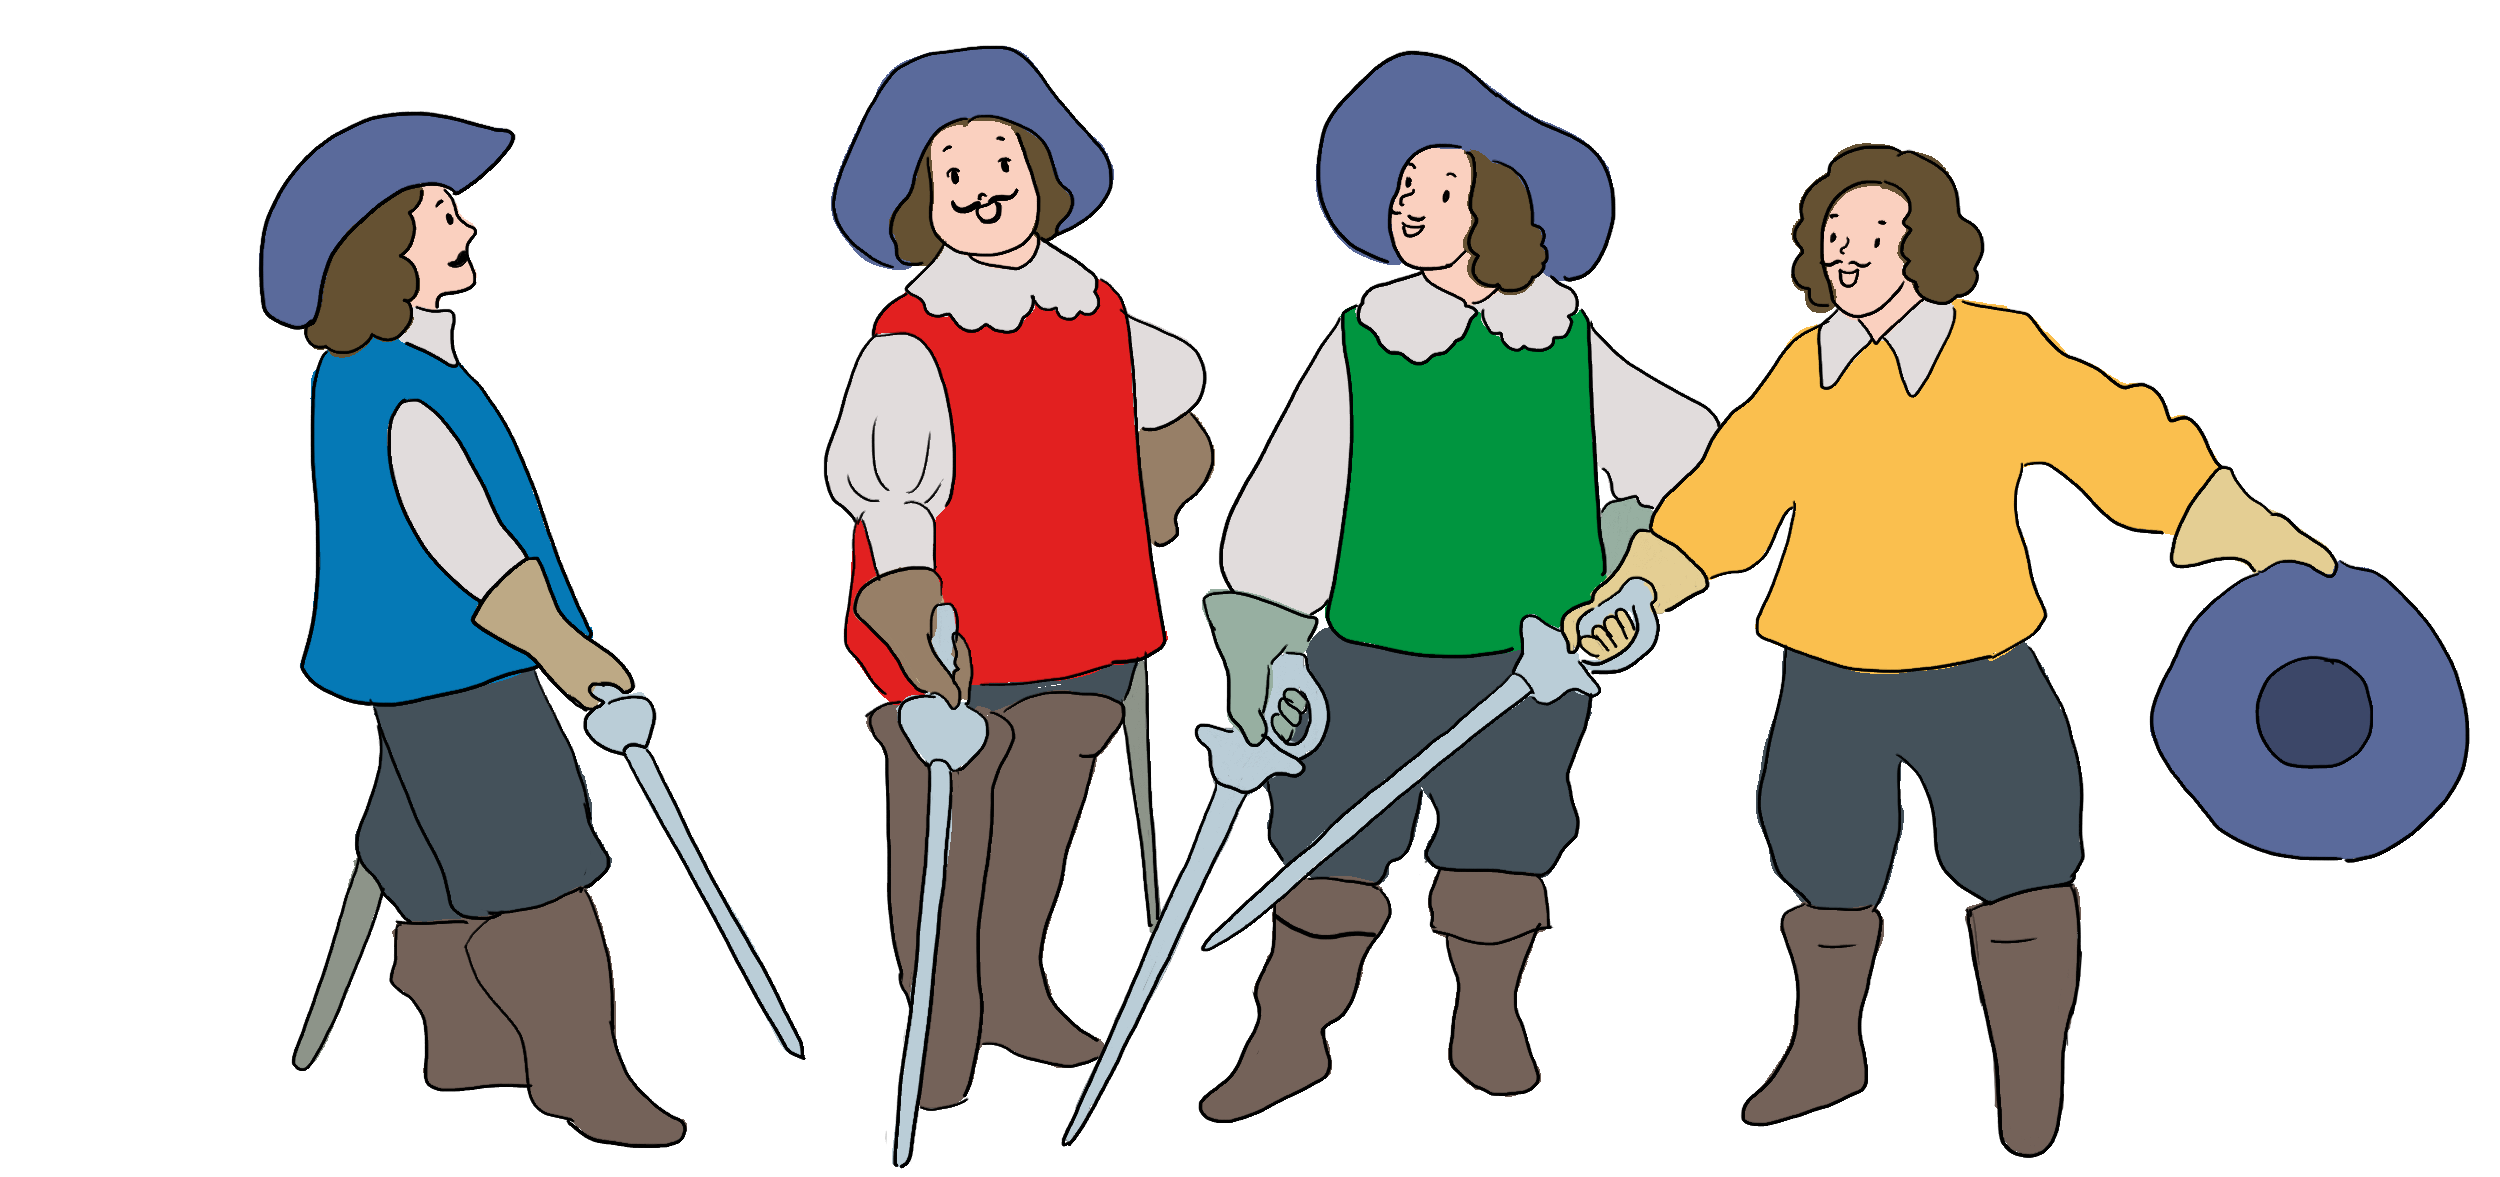
\includegraphics[width=1\linewidth]{Pi3_bai5}
		\vspace*{-15pt}
	\end{figure}
	$\pmb{6.}$ Tại một khách sạn nọ, nhân viên trực quản lý điều hành phải làm việc từ $8$h sáng tới $8$h tối (phương án $A$), hoặc từ $8$h tối tới $8$h sáng (phương án $B$), hoặc làm trọn cả ngày $24$h bắt đầu từ $8$h (sáng hoặc tối) (phương án $C$). Nếu làm theo phương án $A$, nhân viên trực quản lý sẽ được nghỉ không ít hơn $1$ ngày ($24$h). Nếu làm theo phương án $B$, nhân viên trực quản lý sẽ được nghỉ không ít hơn $1$ ngày rưỡi ($36$h). Còn nếu làm theo phương án $C$, nhân viên trực quản lý sẽ được nghỉ không ít hơn hai ngày rưỡi ($60$h).
	\vskip 0.1cm
	Hỏi khách sạn phải cần có ít nhất bao nhiêu nhân viên trực quản lý để đảm bảo lịch làm việc, nghỉ ngơi ở trên được tuân thủ?
\end{multicols}
\vspace*{-10pt}
{\color{toancuabi}\rule{1\linewidth}{0.1pt}}
\begingroup
\AddToShipoutPicture*{\put(110,405){
\includegraphics[scale=1]{../tieude2.pdf}}} 
\centering
\endgroup
\vspace*{75pt}

\begin{multicols}{2}
	$\pmb{1.}$ Hai anh bạn rủ nhau đi câu cá. Khi được hỏi ``Trong mỗi giỏ của các anh có bao nhiêu con cá đấy?" thì anh thứ nhất trả lời ``Trong giỏ của tôi có số cá bằng nửa số cá ở giỏ của anh kia và thêm $10$ con nữa". Anh thứ hai lại nói ``Còn trong giỏ của tôi có số cá bằng số cá trong giỏ của anh kia và thêm $20$ con nữa". Vậy cả hai anh bạn có tất cả bao nhiêu con cá nhỉ? 
	\begin{figure}[H]
		\centering
		\vspace*{-10pt}
		\captionsetup{labelformat= empty, justification=centering}
		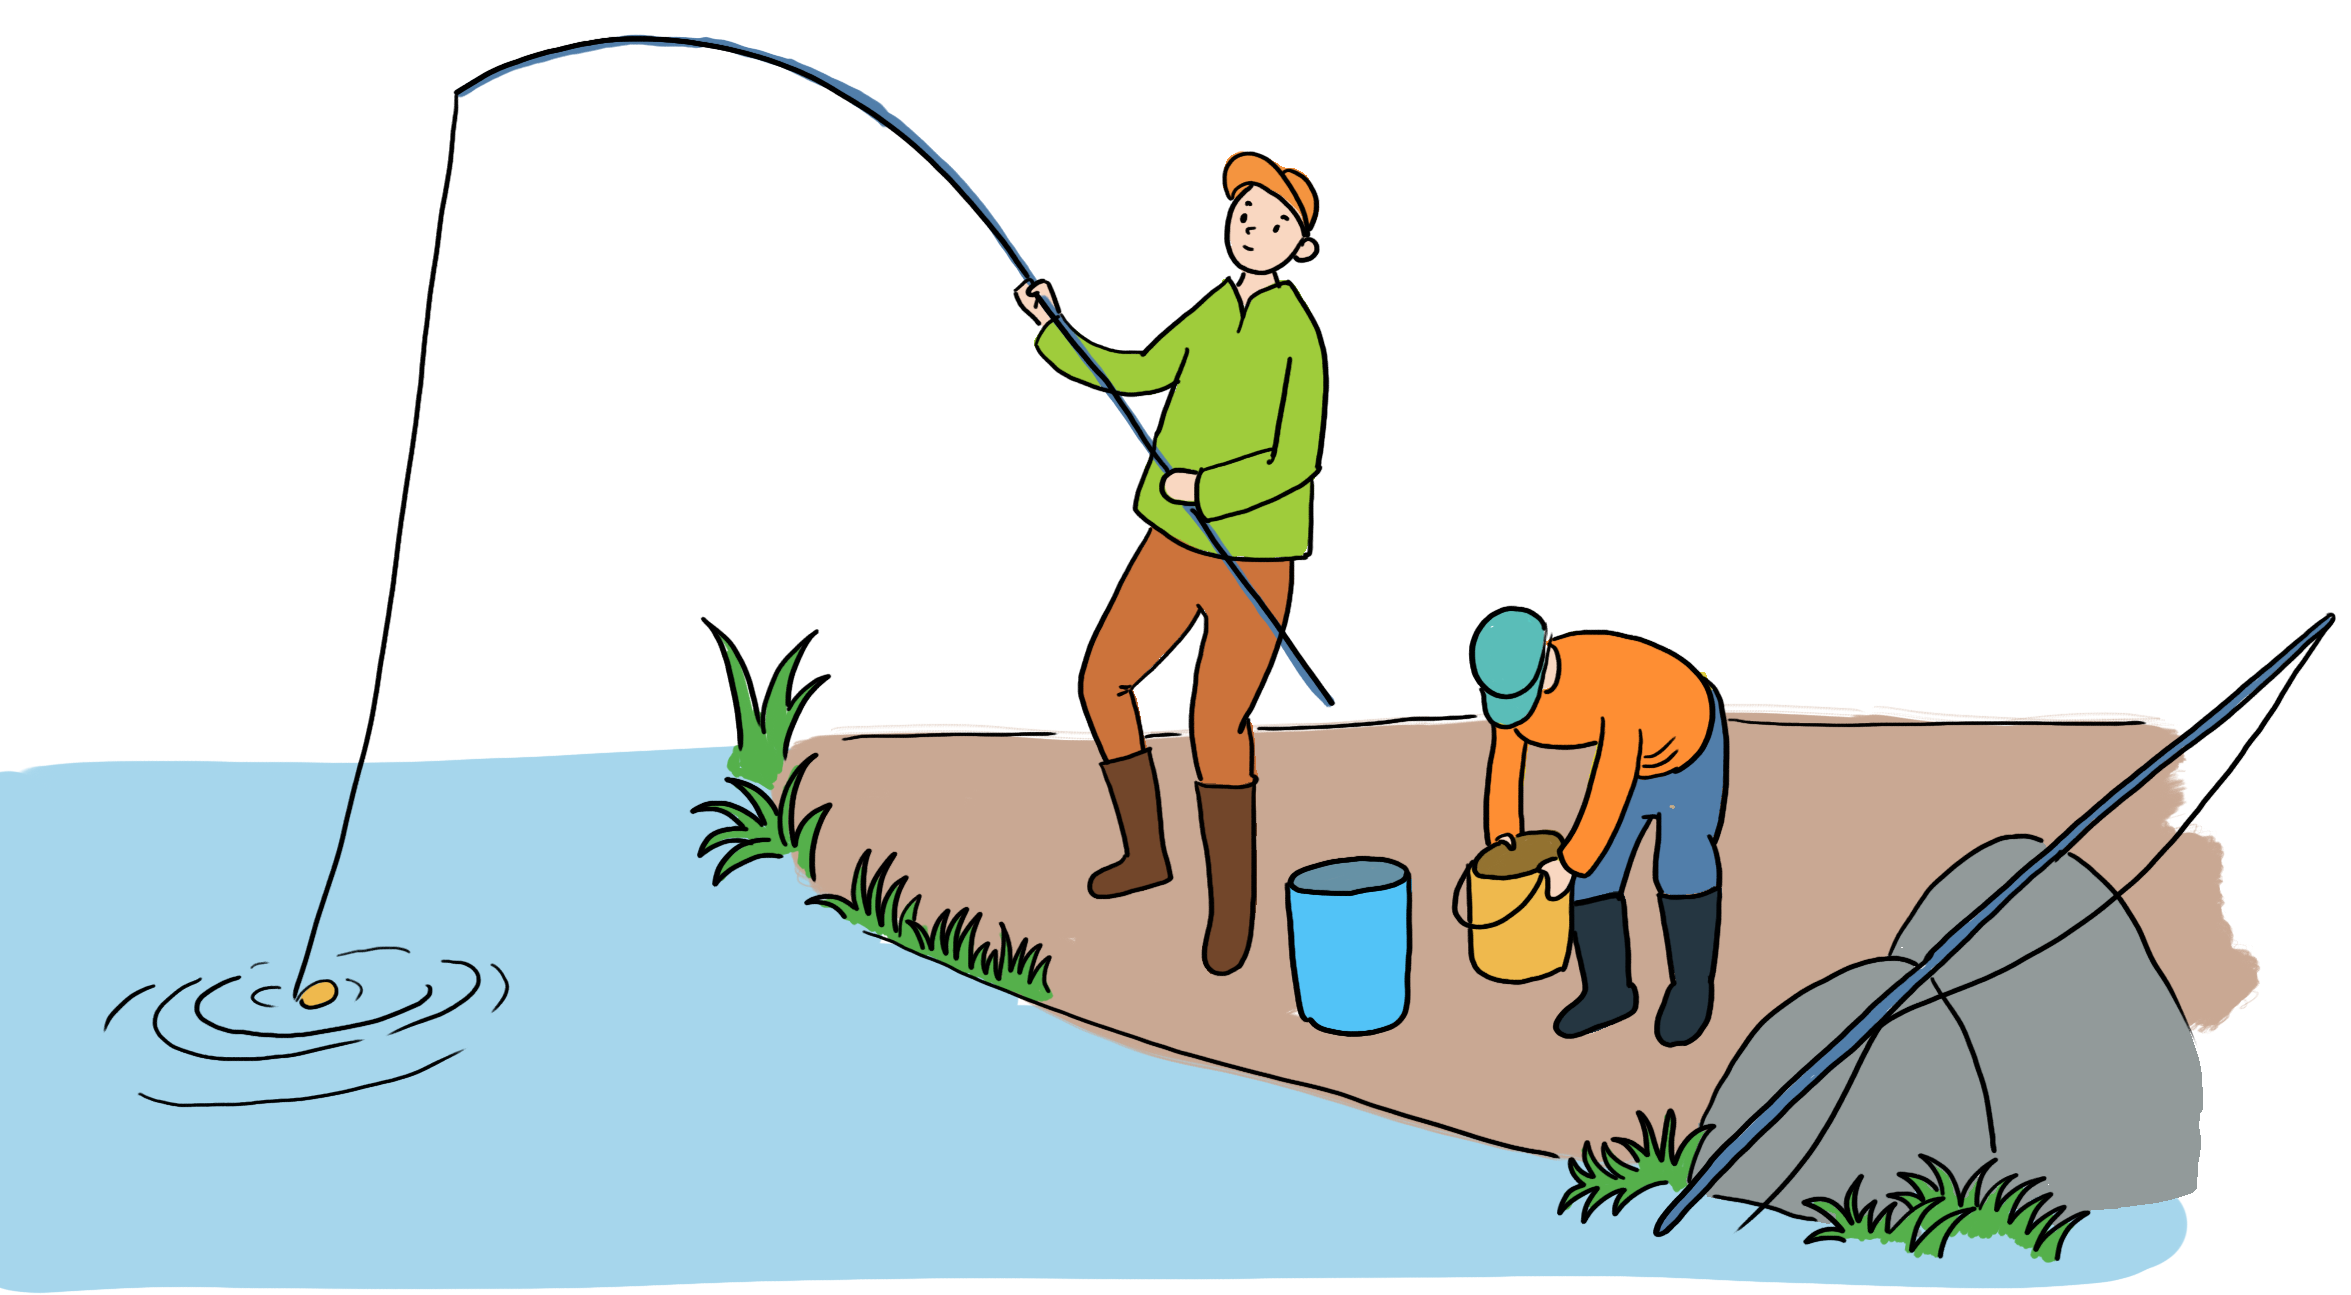
\includegraphics[width=1\linewidth]{Pi10_ToanBi_Bai1}
		\vspace*{-15pt}
	\end{figure}
	\textit{Lời giải.} Một nửa số cá của anh thứ hai sẽ là nửa số cá của anh thứ nhất cộng thêm $10$ con. Vậy nửa số cá của anh thứ hai cộng thêm $10$ con sẽ bằng nửa số cá của anh thứ nhất cộng thêm $20$ con. Theo đề bài, số cá này bằng cả số cá của anh thứ nhất.
	\vskip 0.1cm
	Vậy một nửa số cá của anh thứ nhất là: $20$ (con)
	\vskip 0.1cm
	Suy ra anh thứ nhất có số cá là
	\begin{align*}
		2 \times 20 = 40 \text{  (con)}
	\end{align*}
	và anh thứ hai có số cá là 
	\begin{align*}
		40+20 = 60 \text{  (con).}
	\end{align*} 
	Tổng số cá của cả hai anh là 
	\begin{align*}
		40+60 = 100 \text{  (con).}
	\end{align*}
	Đây là bài tập đơn giản, tuy nhiên các em thử tập làm bằng nhiều cách khác nhau thông qua suy luận thông thường mà không cần dùng tới cách lập phương trình nhé.
	\vskip 0.1cm
	$\pmb{2.}$ Lọ lem có $100$ rổ đựng hạt dẻ, lúc đầu số hạt dẻ trong mỗi rổ là như nhau. Lọ Lem lấy đi trong rổ thứ nhất một số hạt dẻ, lấy từ rổ  thứ hai một số hạt gấp đôi như thế, lấy từ rổ thứ ba một số hạt gấp ba như thế, và cứ như vậy. Cuối cùng thì trong rổ thứ $100$ chỉ còn đúng một hạt dẻ, và còn lại ở tất cả trong $100$ rổ tổng cộng là $14950$ hạt dẻ. Hỏi ban đầu trong mỗi rổ có bao nhiêu hạt dẻ?
	\begin{figure}[H]
		\centering
		\vspace*{-10pt}
		\captionsetup{labelformat= empty, justification=centering}
		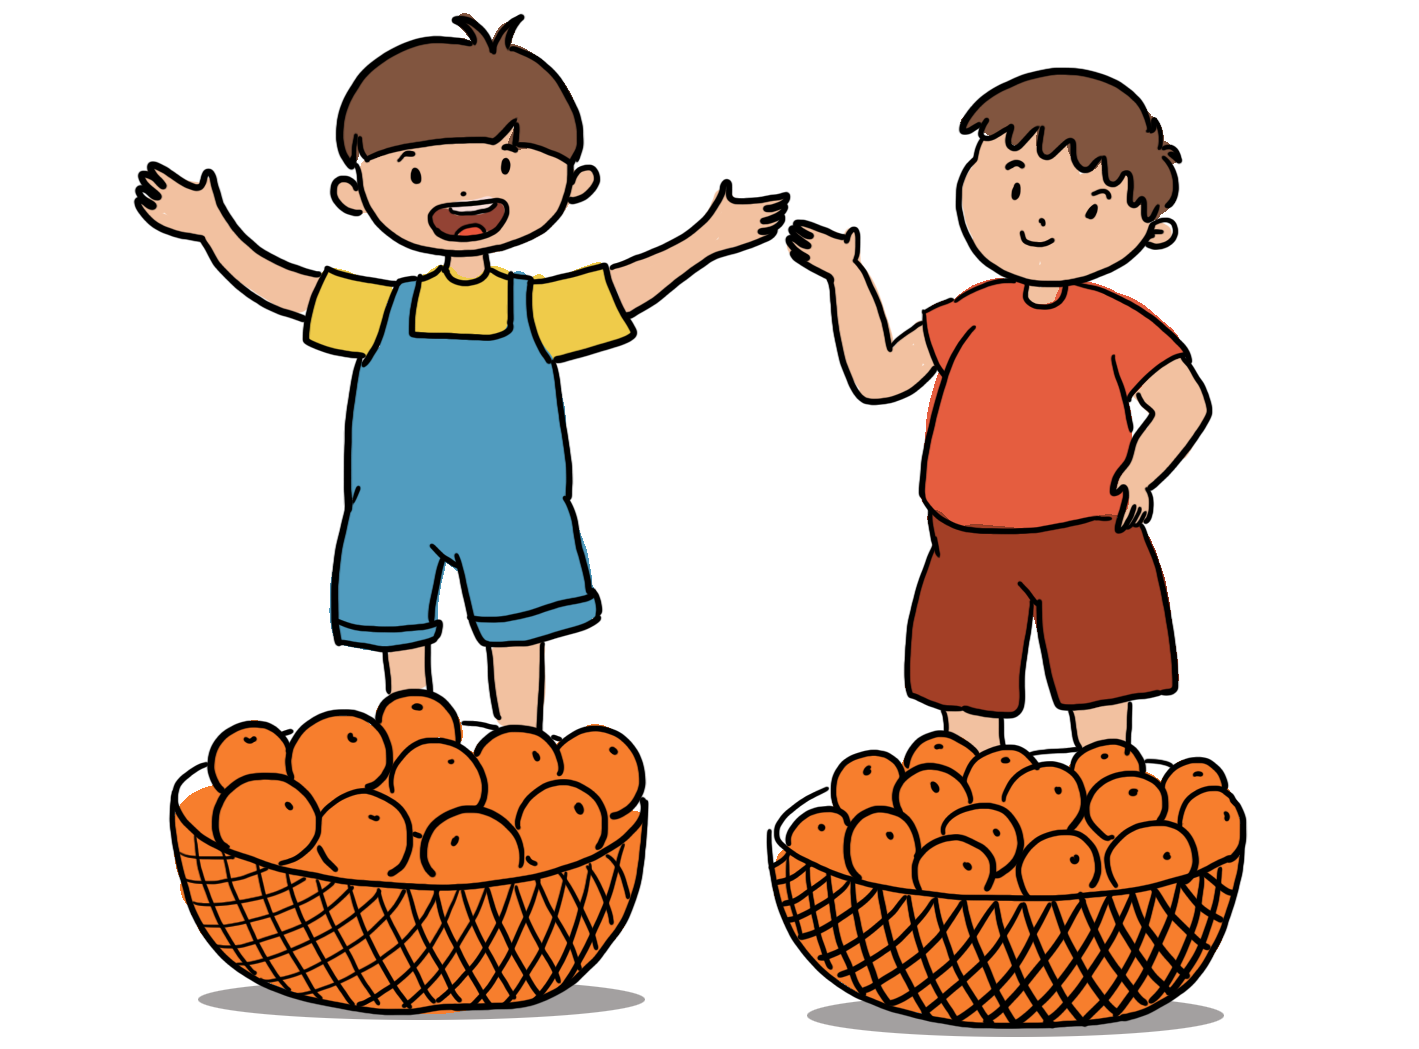
\includegraphics[width=1\linewidth]{Pi10_ToanBi_Bai2}
		\vspace*{-15pt}
	\end{figure}
	\textit{Lời giải.} 	Gọi số hạt dẻ mà Lọ Lem lấy ở rổ thứ nhất là $a$, khi đó tổng cộng số hạt dẻ mà Lọ lem đã lấy đi ở $100$ rổ là
	\begin{align*}
		a+ 2a+\cdots+100a=5050a.
	\end{align*} 
	Do rổ cuối cùng còn lại $1$ hạt dẻ nên ban đầu số hạt dẻ ở rổ cuối cùng (cũng là số hạt dẻ ở các rổ khác) là: $100a+1$ (hạt).
	\vskip 0.1cm
	Vậy, ban đầu tổng số hạt dẻ là
	\begin{align*}
		100\times(100a+1) = 10000a+100 \text{  (hạt).}
	\end{align*} 
	Ta có hệ thức là: $10000a+100-5050 a =14950$. Từ đó suy ra $a=3$. Vì vậy ban đầu mỗi rổ có  $100\times 3+1 = 301$ hạt dẻ.
	\vskip 0.1cm
	$\pmb{3.}$ Hai bạn học sinh là Nam và Vũ gặp nhau tại nhà của Vũ. Nam nói ``Nếu lấy số nhà của tớ là một số có hai chữ số trừ đi số có hai chữ số tạo thành khi viết theo thứ tự ngược lại, thì sẽ ra số nhà của cậu. Vậy tớ sống ở số nhà nào?"
	\vskip 0.1cm
	Vũ trả lời ``Ôi, bài toán này dễ quá" -- và giải ra luôn đáp số.
	\vskip 0.1cm
	Vậy các bạn đó sống ở những số nhà nào nhỉ?
	\vskip 0.1cm
	\textit{Lời giải.} 	Nếu thực hiện phép trừ của Nam, ta sẽ nhận được số có dạng $9\times k$, ở đó $k$ là hiệu của chữ số hàng chục và chữ số hàng đơn vị. Vì số viết theo thứ tự ngược lại cũng là số có hai chữ số, nên $k\le8$. 
	\vskip 0.1cm
	Nếu $k<8$ thì có thể thấy có nhiều số có hai chữ số (là số nhà) mà sau khi làm phép tính trừ đã cho sẽ cho kết quả như nhau. Khi đó Vũ không thể giải được ngay câu đố của Nam. Do đó $k=8$. Các em có thể tìm thấy số nhà của Nam là $91$, và số nhà của Vũ là $72$.
	\begin{figure}[H]
		\centering
		\vspace*{-5pt}
		\captionsetup{labelformat= empty, justification=centering}
		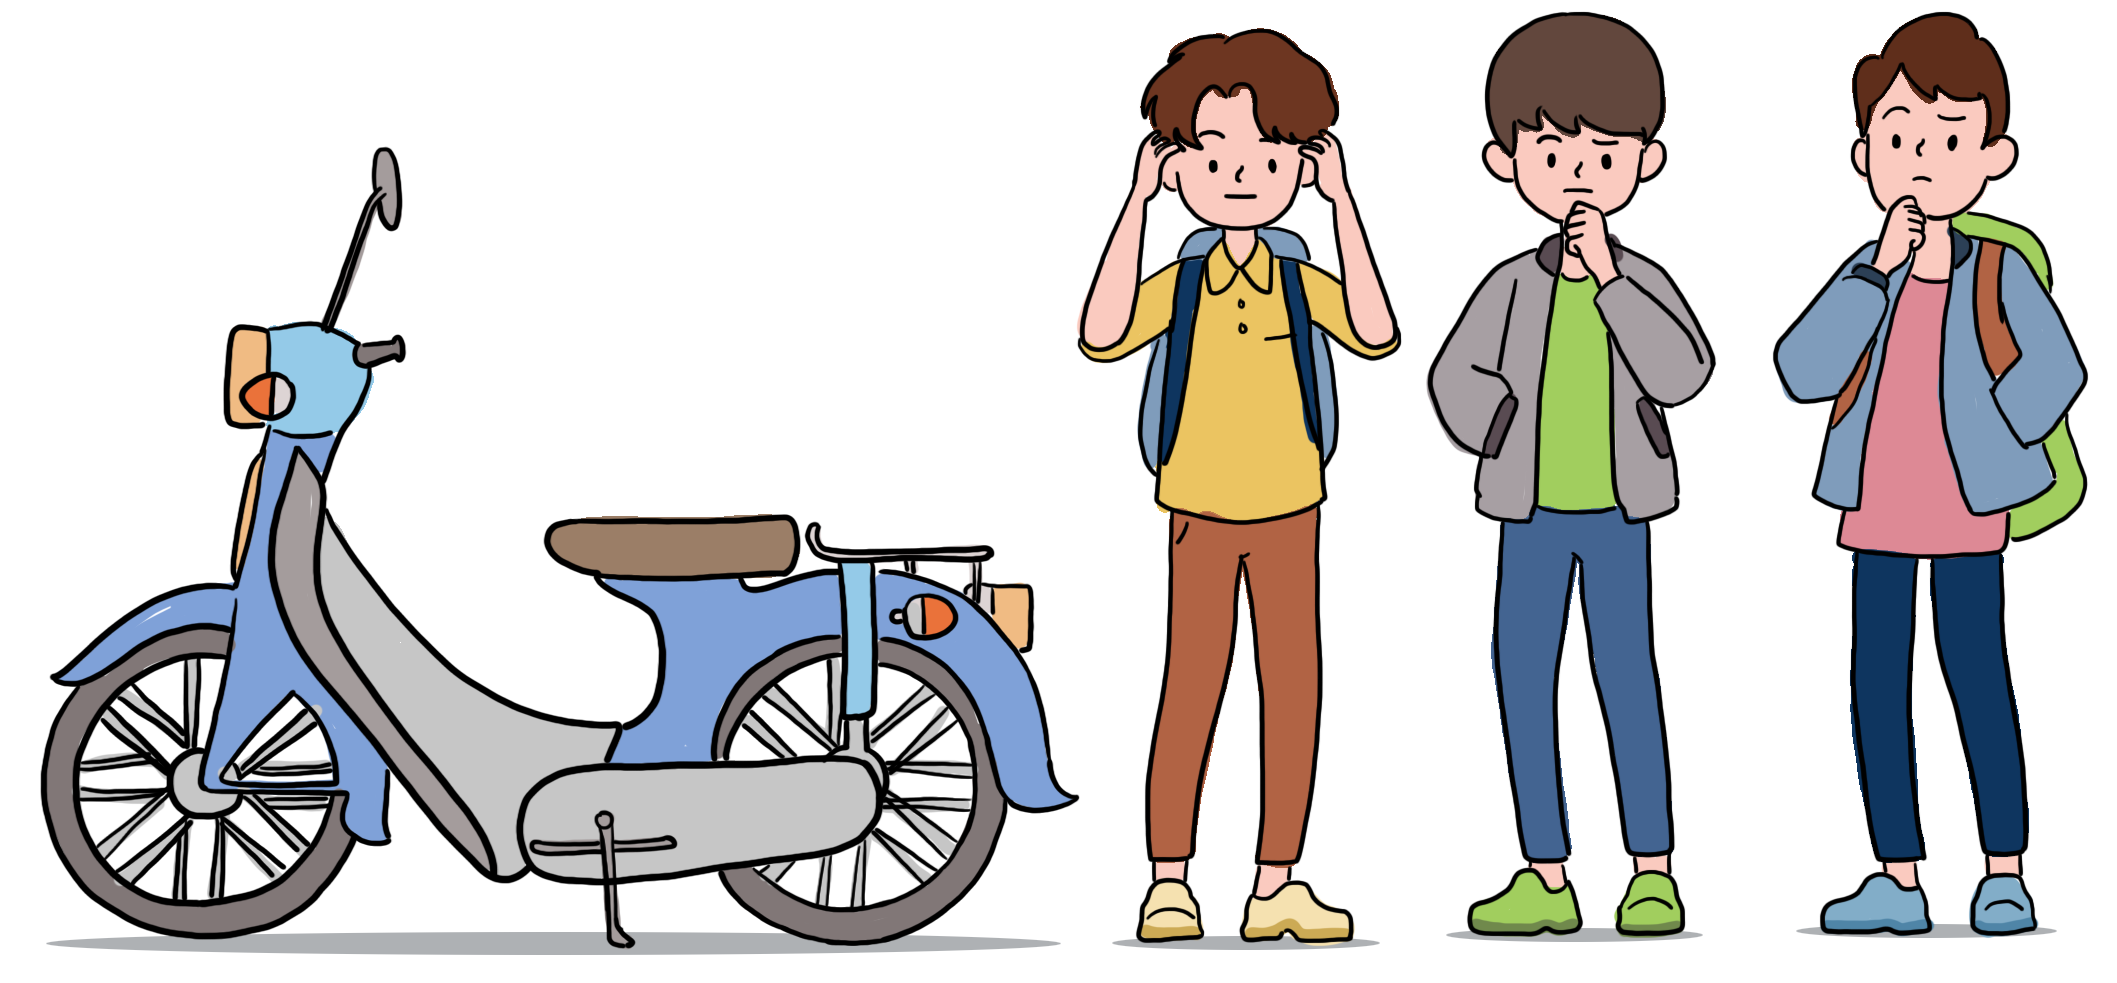
\includegraphics[width=1\linewidth]{Pi10_ToanBi_Bai3}
		\vspace*{-15pt}
	\end{figure}
	$\pmb{4.}$ Lớp của Hùng có $35$ học sinh. Trong số đó có $20$ em tham gia câu lạc bộ Toán, $11$ em tham gia câu lạc bộ Khéo tay, $10$ em không tham gia vào hai nhóm này. Hỏi có tất cả bao nhiêu em vừa tham gia CLB Toán lại vẫn không quên tham gia cả CLB Khéo tay nhỉ?
	\begin{figure}[H]
		\centering
		\vspace*{-5pt}
		\captionsetup{labelformat= empty, justification=centering}
		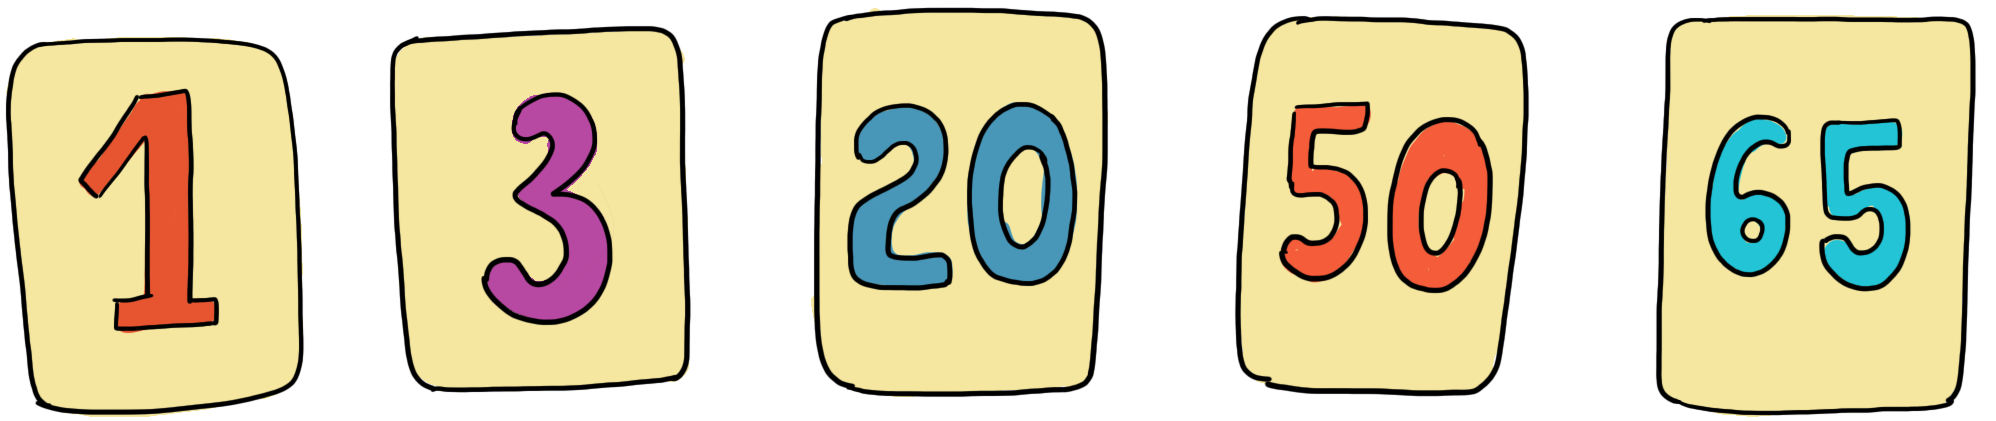
\includegraphics[width=1\linewidth]{Pi10_ToanBi_Bai4}
		\vspace*{-15pt}
	\end{figure}
	\textit{Lời giải.} 	Chúng ta chia toàn bộ số học sinh trong lớp thành bốn danh sách, mà không có em nào ở trong hai danh sách khác nhau, như sau. Danh sách ``toán thuần tuý" gồm các bạn chỉ tham gia CLB Toán, danh sách ``khéo tay thuần tuý" gồm các bạn chỉ tham gia CLB Khéo tay, danh sách ``giỏi toán lại khéo tay" gồm các bạn tham gia cả $2$ CLB  và cuối cùng là danh sách ``rảnh rỗi" là các bạn không tham gia vào hai CLB này. Theo đề bài, danh sách ``rảnh rỗi" có $10$ bạn, vì thế có $25$ bạn không ``rảnh rỗi". Trong số $25$ bạn này có $20$ bạn tham gia nhóm Toán, vì thế số ``khéo tay thuần tuý" là $5$ bạn. Vậy số bạn vừa tham gia nhóm Toán lại ``khéo tay" nữa là 
	\begin{align*}
		11-5 = 6 \text{ (bạn).}
	\end{align*}
	$\pmb{5.}$ Tùng đến trường mới có nhiều chuyện rất vui nên về khoe với bạn bè.
	\begin{figure}[H]
		\centering
		%		\vspace*{5pt}
		\captionsetup{labelformat= empty, justification=centering}
		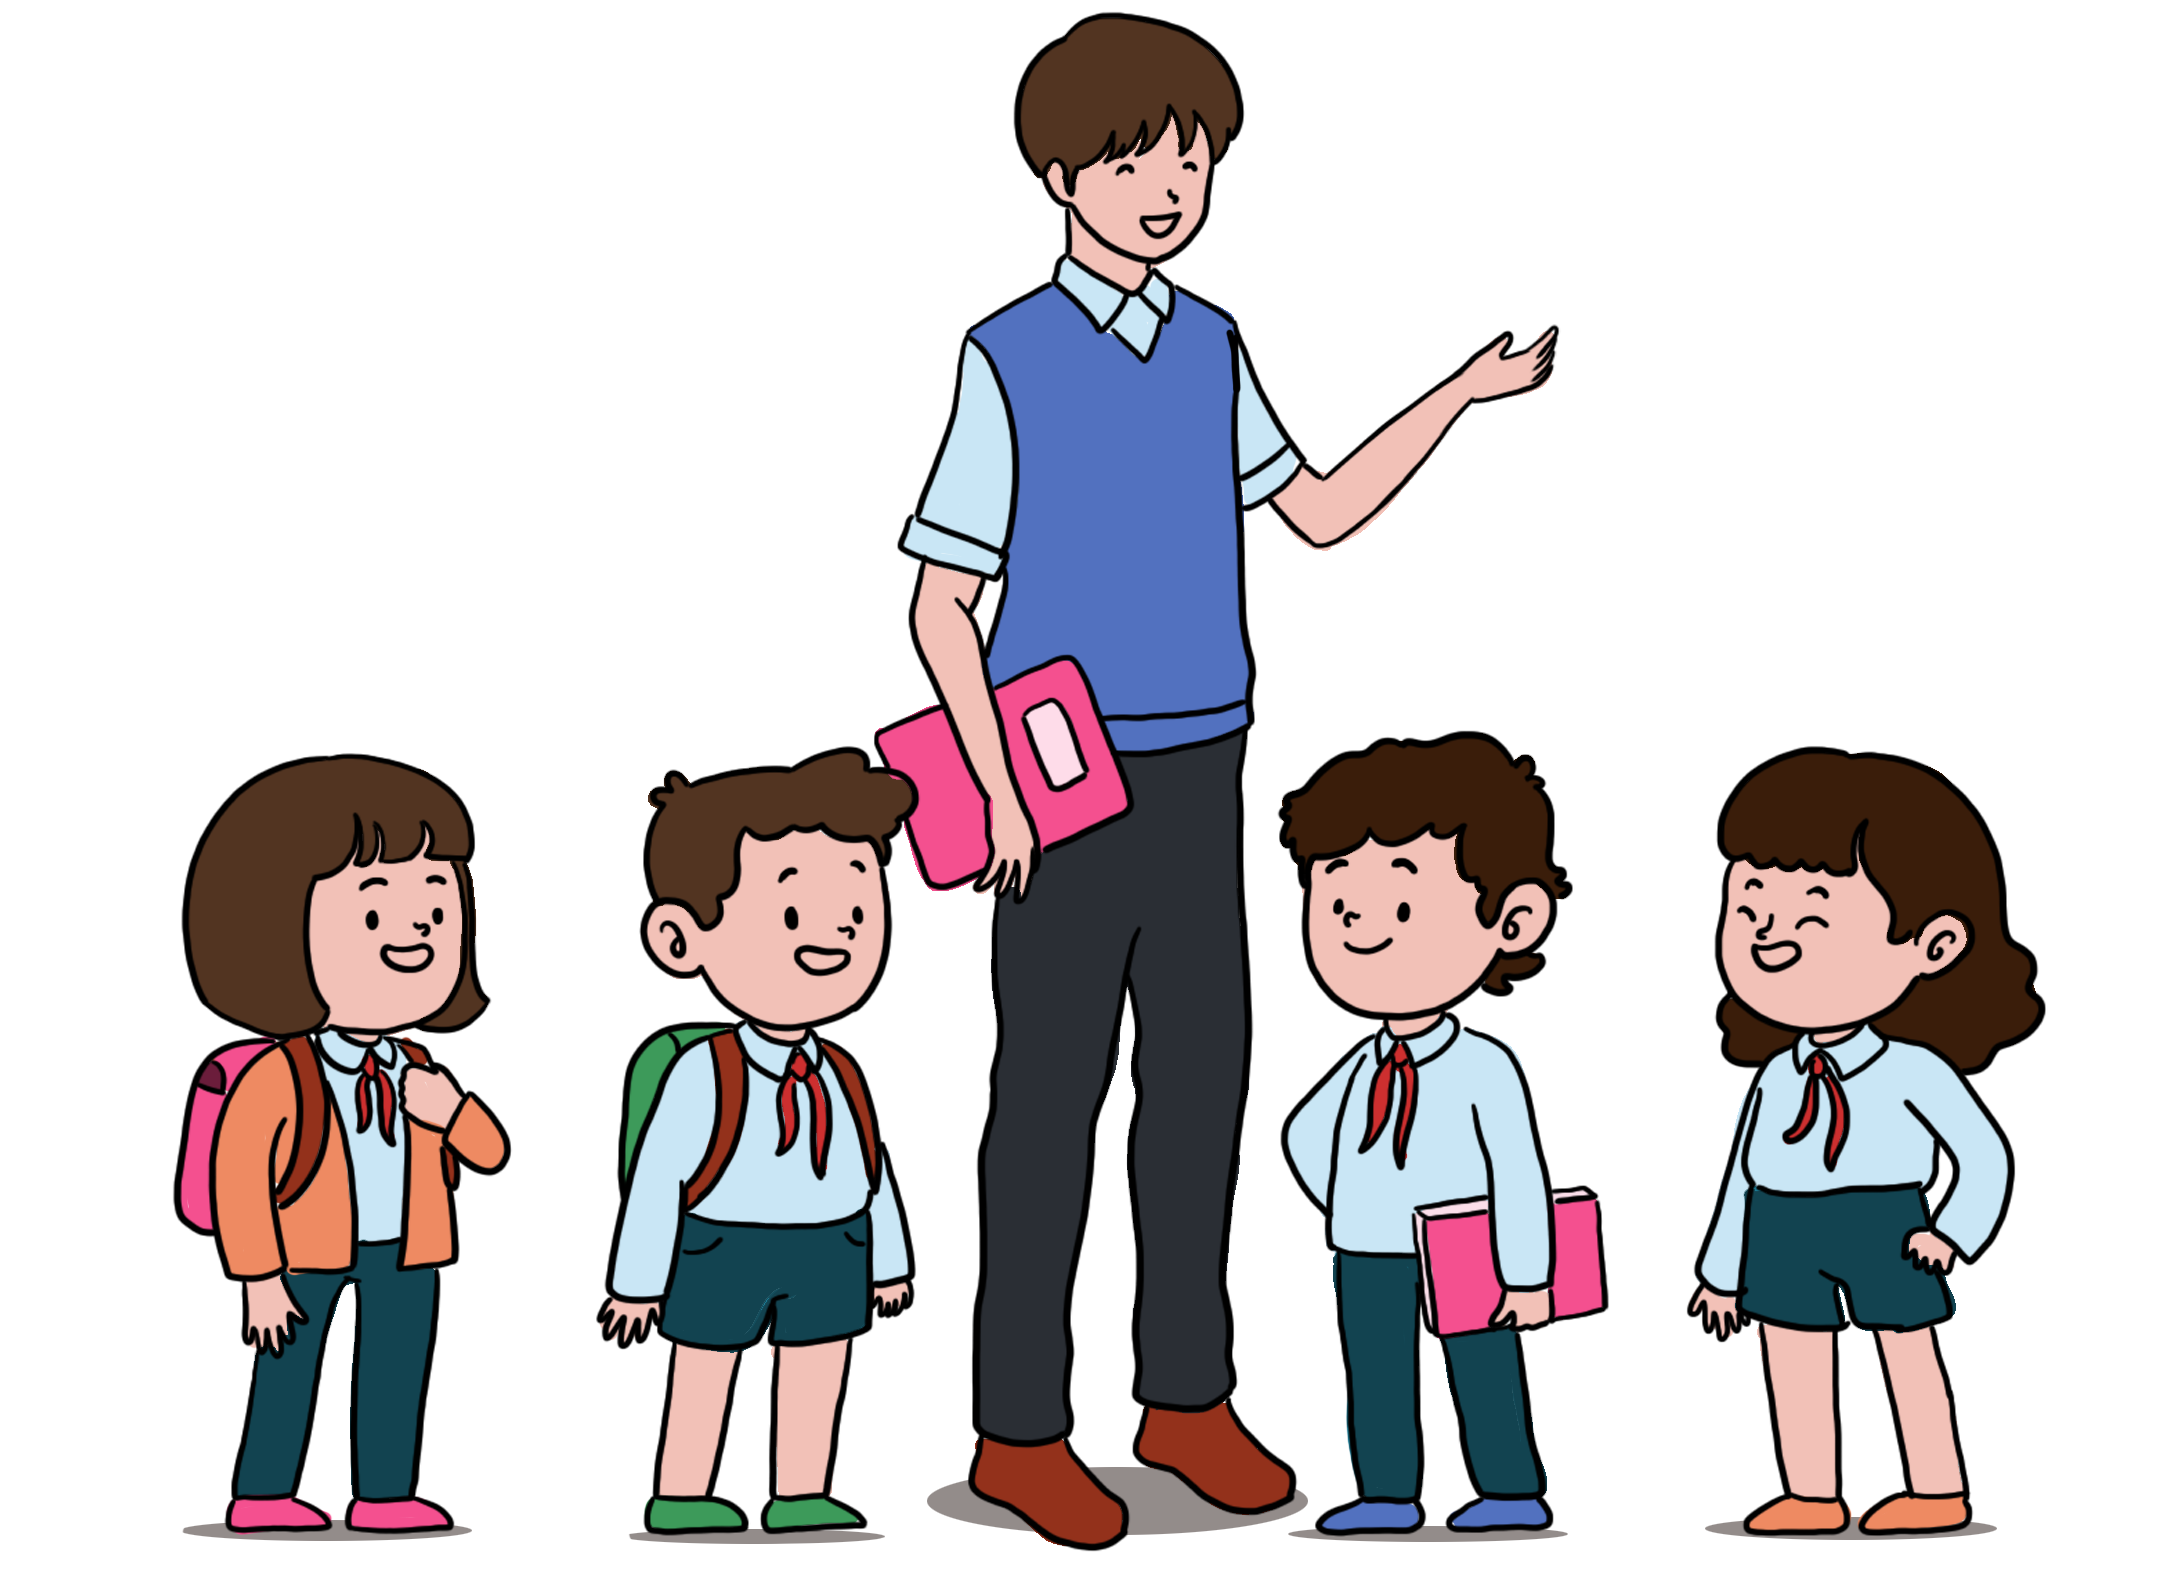
\includegraphics[width=1\linewidth]{Pi10_ToanBi_Bai5}
		\vspace*{-15pt}
	\end{figure}
	-- Lớp tớ có $35$ học sinh. Và các cậu có tưởng tượng được không, mỗi người lại kết bạn với đúng $11$ học sinh cùng lớp.
	\vskip 0.1cm
	-- Không thể thế được! Bách, người bạn thân của Tùng vừa đạt giải trong một cuộc thi Olympic, ngay lập tức trả lời.
	\vskip 0.1cm
	Vì sao Bách lại nghĩ như vậy nhỉ?
	\vskip 0.1cm
	\textit{Lời giải.} 	Ta biểu diễn mỗi học sinh bằng một điểm trên mặt phẳng. Nếu hai học sinh kết bạn với nhau ta sẽ nối hai điểm tương ứng bởi một đoạn thẳng. Như vậy có $35$ điểm, mỗi điểm được nối đúng với $11$ điểm khác. Khi đó tổng số các đầu của các đoạn thẳng nối quan hệ bạn bè là $35\times11$ là một số lẻ. Điều này là vô lý do mỗi đoạn thẳng thể hiện quan hệ bạn bè có đúng hai điểm đầu mút. 
	\vskip 0.1cm
	$\pmb{6.}$ Có $55$ em học sinh tham gia một cuộc thi Olympic. Tất cả các em đều nộp bài. Khi chấm bài, mỗi câu hỏi được chấm bởi một trong ba loại điểm: điểm ``$+$" nếu câu hỏi được trả lời hoàn toàn đúng; điểm ``$-$" nếu câu hỏi đã có trả lời nhưng chưa ra đúng đáp số; và điểm ``$0$" nếu câu hỏi chưa được trả lời. Sau khi chấm toàn bộ bài thi, ban tổ chức thấy không có hai bài thi nào có cả các số điểm ``$+$" và số điểm ``$-$" đồng thời trùng nhau. Vậy trong kỳ thi Olympic đó phải có ít nhất bao nhiêu câu hỏi?
	\vskip 0.1cm
	\textit{Lời giải.} 	Giả sử $a$ là số câu hỏi được ra.  Ta chia ra các trường hợp sau
	\vskip 0.1cm
	$1.$ Bài thi có tất cả các câu hỏi đều được trả lời: Khi đó số các bài thi sẽ không vượt quá $a+1$ bài: từ bài có $a$ dâú ``$+$" và $0$ dấu ``$-$" cho đến bài có $0$ dấu ``$+$" và $a$ dấu ``$-$".  
	\vskip 0.1cm
	Bài thi trong đó chỉ có đúng một bài chưa có trả lời (có một điểm ``$0$"): Số các bài thi  nhiều nhất là $a$ bài (từ $a-1$ điểm ``$+$" và $0$ điểm ``$-$" cho đến bài có $0$ điểm ``$+$" và $a-1$ điểm ``$-$"). $\ldots$
	\vskip 0.1cm
	Và cứ xét như vậy, ta thấy tổng số các bài thi nhiều nhất là 
	\begin{align*}
		(a\!+\!1)\!+\!a\!+\!(a\!-\!1)\!+\!\cdots\!+\!1=\dfrac{(a\!+\!1)(a\!+\!2)}{2}.
	\end{align*}
	Từ đó ta có $55\le\dfrac{(a+1)(a+2)}{2}$. Với $a=9$ ta có $\dfrac{10\cdot11}{2}=55$. Vậy là $a \ge 9$. 
	\vskip 0.1cm
	Vì vậy số câu hỏi ít nhất được ra là $9$ câu.
\end{multicols}
\newpage
\begingroup
\thispagestyle{toancuabinone}
\blfootnote{$^1$\color{toancuabi}Ottawa, Canada.}
\AddToShipoutPicture*{\put(60,733){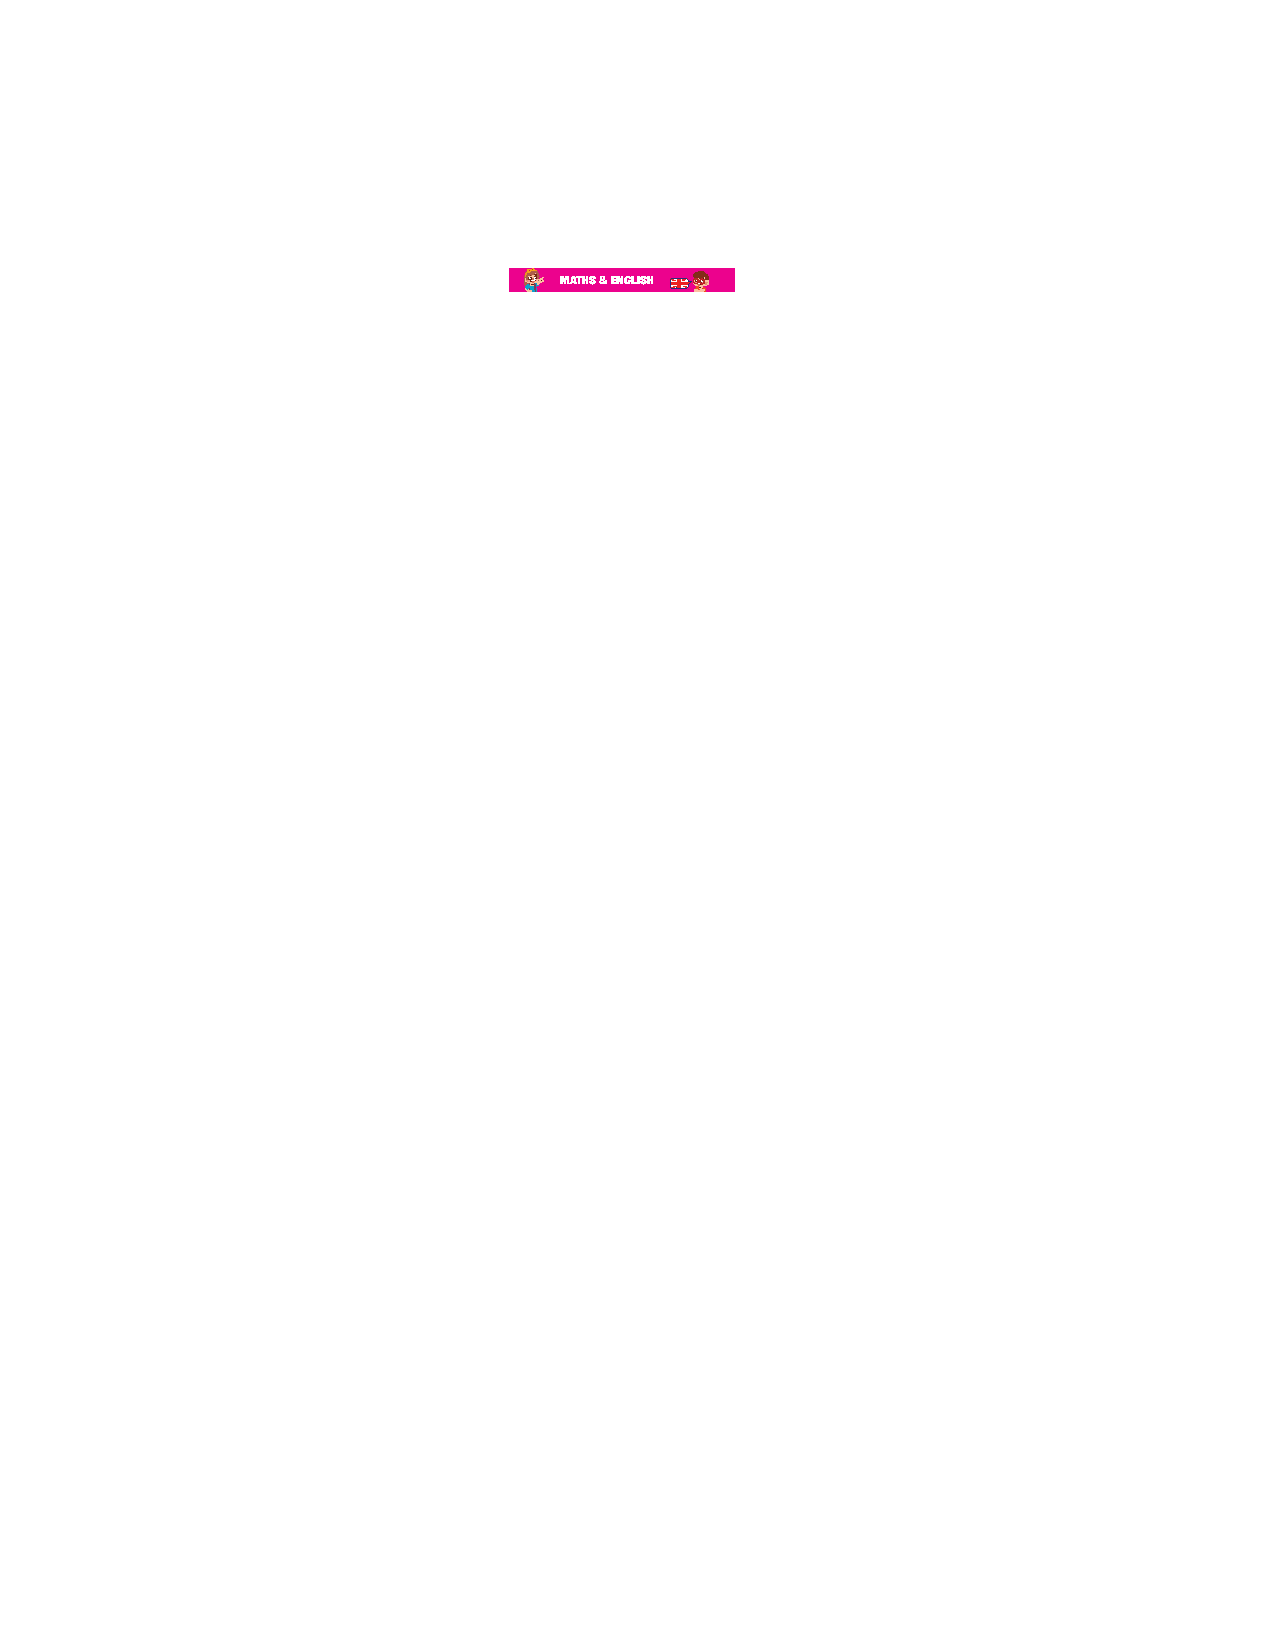
\includegraphics[width=17.2cm]{../mathc.pdf}}}
%\AddToShipoutPicture*{\put(-2,733){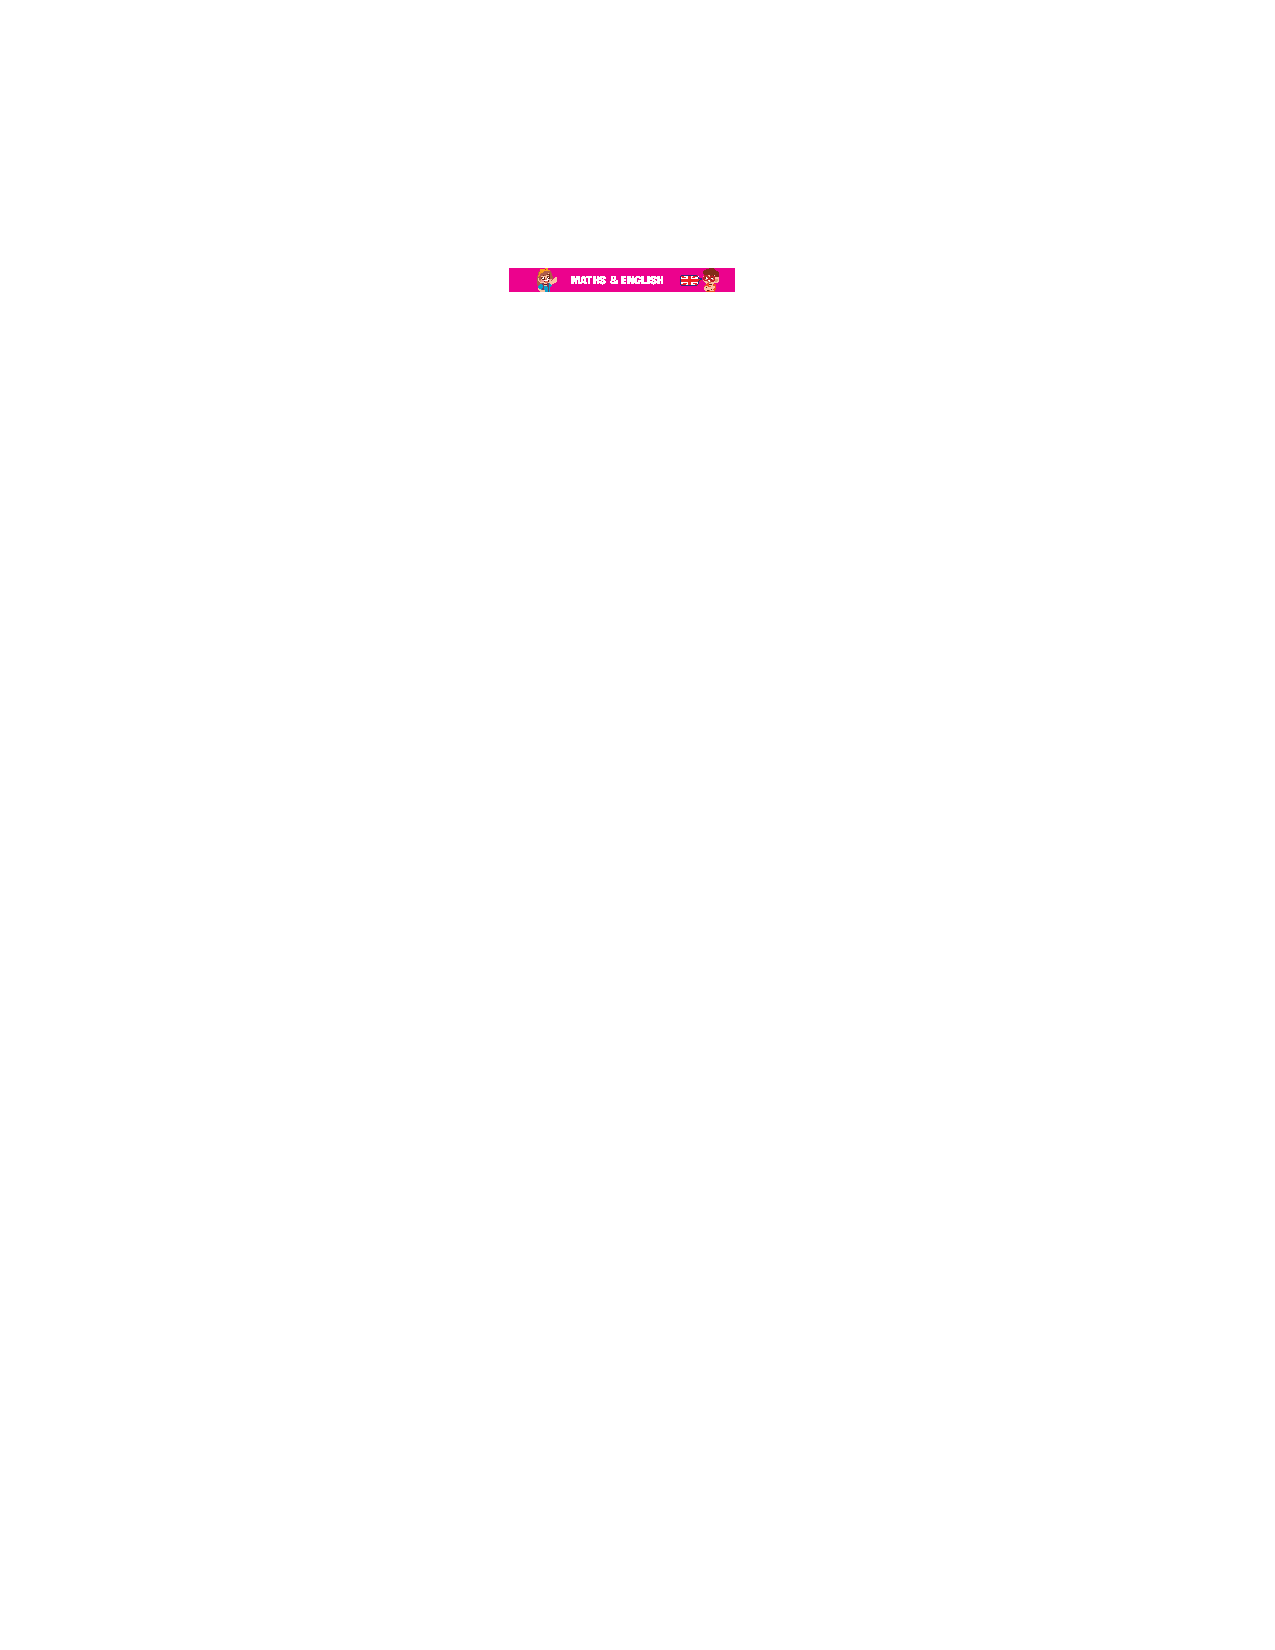
\includegraphics[width=17.2cm]{../mathl.pdf}}} 
\AddToShipoutPicture*{\put(145,673){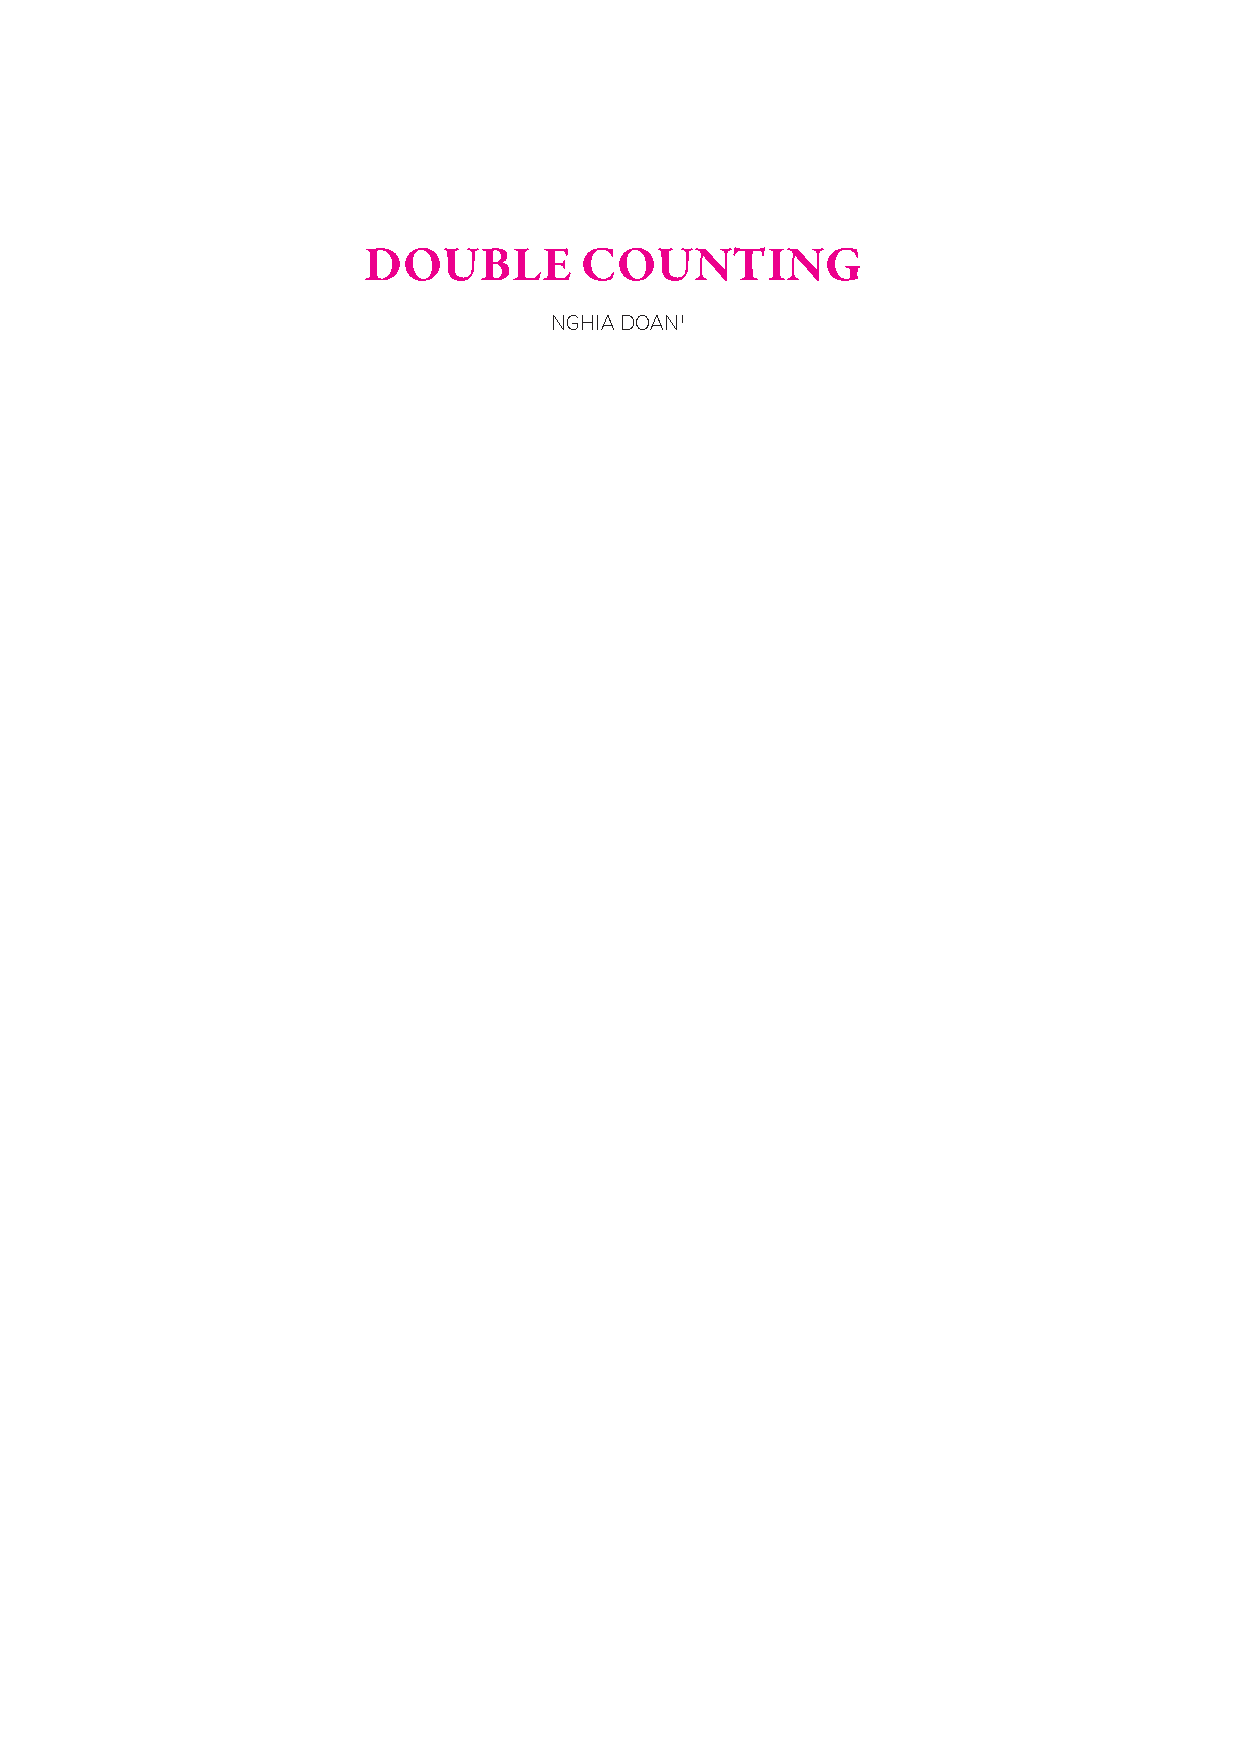
\includegraphics[scale=1]{../tieude6.pdf}}} 
\centering
\endgroup
\graphicspath{{../toancuabi/pic/}}
\vspace*{33pt}

\begin{multicols}{2}
	In this article, we introduce some problems which can be solved by the method of double counting. In other words, we will count a quantity in two different ways.
	\vskip 0.2cm
	\PIbox{\textbf{\color{toancuabi}Example} (Areas)\textbf{\color{toancuabi}.}
		Let $ABCD$ be a parallelogram. Let $E$ and $F$ be two points on the line segments $AB$ and $BC$ respectively. The lines $AF,CE,DE$ and $DF$ divide the parallelogram into $8$ different regions, the areas of which are written in the figure. 
		\vskip 0.1cm
		Find the sum of the areas $a+b+c$.}
	\begin{figure}[H]
		\centering
		\vspace*{-5pt}
		\captionsetup{labelformat= empty, justification=centering}
		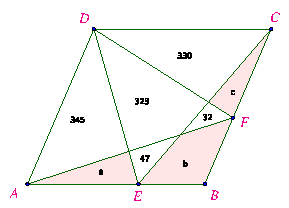
\includegraphics[width=1\linewidth]{hc-2022-2-2-6.pdf}
		\vspace*{-10pt}
	\end{figure}
	\textit{Solution.}
	From the properties of the parallelogram $ABCD,$ the following triangle pairs, with the same base and height, have the same area
	\begin{align*}
		\left.
		\begin{aligned}
			[AFB] = [DFB]\\
			[CEB] = [DEB]
		\end{aligned}
		\right\}
		\Rightarrow& [AFB] + [CEB] \\
		&= [DFB] + [DEB] \\
		&= [DEBF]
	\end{align*}
	Therefore
	\begin{align*}
		&(a + 47 + b) + (c + 32 + b)\\
		= \,&(323 + 47 + b + 32)\\
		\Rightarrow\, &a + b + c = 323.
	\end{align*}
	\vspace*{0.1pt}
	
	\vspace*{-6pt}
	\PIbox{\textbf{\color{toancuabi}Example} (How many knights are needed to protect King Anthony?)\textbf{\color{toancuabi}.}
		King Anthony went hunting with his knights.
		At night, they stayed in one of the king's hunting lodges in the forest.
		In this house, there are nine rooms. The king slept in the central room.
		The knights stayed in the eight surrounding rooms such that
		in each direction north, south, east, west the total number of knights 
		in the \textit{three rooms} facing that direction should always be \textit{nine}.
		\textit{For example, the diagram below shows a possible case with each room has 3 knights.
			The letter $K$ denotes the King staying in the central room.}
		\begin{table}[H]
			\vspace*{-5pt}
			\centering
			\captionsetup{labelformat= empty, justification=centering}
			\renewcommand{\arraystretch}{1.2}
			\begin{tabular}{|c|c|c|}
				\hline
				$3$ & $3$    & $3$ \\ \hline
				$3$ & K & $3$ \\ \hline
				$3$ & $3$    & $3$ \\ \hline
			\end{tabular}
			\vspace*{-5pt}
		\end{table}
		What is the smallest possible number of knights? What is the largest?}
	\vskip 0.1cm
	\textit{Solution.}
	Let $a_1,a_2,a_3,a_4,b_1,b_2,b_3,$ and $b_4$ be the numbers of knights in each room as shown in the diagram below.
	Let $S=a_1+a_2+a_3+a_4+b_1+b_2+b_3+b_4$. We have:
	\begin{align*}
		&36 = (a_1\!+\!b_1\!+\!a_2)\!+\!(a_2\!+\!b_2\!+\!a_3)\\
		&\quad\quad\!+\!(a_3\!+\!b_4\!+\!a_4)\!+\!(a_4\!+\!b_4\!+\!a_1)\\
		\Rightarrow&
		\begin{cases}
			S = 36 - (a_1+a_2+a_3+a_4)\\
			S = \dfrac{1}{2}\left(36 + (b_1+b_2+b_3+b_4)\right)
		\end{cases}
	\end{align*}
	\begin{table}[H]
		\vspace*{-5pt}
		\centering
		\captionsetup{labelformat= empty, justification=centering}
		\begin{tabular}{|c|c|c|}
			\hline
			$a_1$ & $b_1$ & $a_2$ \\ \hline
			$b_4$ & K & $b_2$ \\ \hline
			$a_4$ & $b_3$ & $a_3$ \\ \hline
		\end{tabular}
		\caption{\small\textit{\color{toancuabi}With variables}}
		\vspace*{-10pt}
	\end{table}
	Thus, the smallest possible value of $S$ is $18$, if $b_1=b_2=b_3=b_4=0$ and $a_1=a_3=5,a_2=a_4=4.$
	The largest value of $S$ is $36$, if $a_1=a_2=a_3=a_4=0$ and $b_1=b_2=b_3=b_4=9.$
	\vskip 0.2cm
	\PIbox{\textbf{\color{toancuabi}Example} (What are the family names of the sisters?)\textbf{\color{toancuabi}.}
		Four pairs of brother--sister share $32$ cookies.
		Among the sisters, Lan got one, Mai got two, Na got three, and Quynh got four cookies.
		Danny Tran took as many as his sister, Elvin Nguyen twice as many as his sister,
		Franklin Pham three times as his sister, and Williams Quach four times as many as his sister.
		\vskip 0.1cm
		What are the family names of the girls?}
	\vskip 0.2cm
	\textit{Solution.}
	Let $x, 2y, 3z$ and $4w$ be the numbers of cookies that 
	Danny Tran, Elvin Nguyen, Franklin Pham and Williams Quach took.
	Their sisters took $x, y, z$ and $w$ cookies respectively. Therefore,
	\begin{align*}
		&x + 2y + 3z + 4w + x + y + z + w = 32\\
		\Rightarrow &2x + 3y + 4z + 5w = 32.
	\end{align*}
	Note that $x, y, z, w$ form a permutation of $1,2,3,4,$ so $x + y + z + w = 10.$
	Therefore
	\begin{align*}
		&-x + z + 2w \!=\! 32-3(x + y + z + w) \!=\! 2 \\
		\Rightarrow \,&x > z, x \text{\ and\ } z \text{\ have the same parity}\\
		\Rightarrow\,&-x+z=-2 \Rightarrow  w=2 \\
		\Rightarrow \,&x=3, z=1, y=4. 
	\end{align*}
	Now, Lan got one, Mai got two, Na got three, and Quynh got four cookies.
	\vskip 0.1cm
	$x=3,$ so the girl who took three cookies, Na, is the sister of Danny Tran, hence she is Na Tran.
	\vskip 0.1cm
	$y=4,$ so the girl who took four cookies, Quynh, is the sister of Elvin Nguyen, hence she is Quynh Nguyen.
	\vskip 0.1cm
	$z=1,$ so the girl who took one cookie, Lan, is the sister of Franklin Pham, hence she is Lan Pham.
	\vskip 0.1cm
	$w=2,$ so the girl who took two cookies, Mai, is the sister of Williams Quach, hence she is Mai Quach.
	\vskip 0.1cm
	Thus, the girls' names are Na Tran, Quynh Nguyen, Lan Pham and Mai Quach.
	\vskip 0.2cm
	\PIbox{{\centerline{\color{toancuabi}\textbf{Vocabulary}}}
		\vskip 0.1cm
		{\color{toancuabi}Area:} (dt), diện tích
		\vskip 0.1cm 
		{\color{toancuabi}Base:} (dt) đáy
		\vskip 0.1cm
		{\color{toancuabi}Case:} (dt) trường hợp
		\vskip 0.1cm
		{\color{toancuabi}Cookie:} (dt) bánh
		\vskip 0.1cm
		{\color{toancuabi}Counting:} (dt) đếm, {\color{toancuabi}double counting:} đếm  bằng hai cách
		\vskip 0.1cm
		{\color{toancuabi}Direction:} (dt) hướng
		\vskip 0.1cm
		{\color{toancuabi}Diagram:} (dt) sơ đồ
		\vskip 0.1cm
		{\color{toancuabi}East:} (dt) hướng Đông
		\vskip 0.1cm
		{\color{toancuabi}Figure:} (dt) hình
		\vskip 0.1cm
		{\color{toancuabi}Height:} (dt) chiều cao
		\vskip 0.1cm
		{\color{toancuabi}Hunt:} (đt) săn bắn 
		\vskip 0.1cm
		{\color{toancuabi}Knight:} (dt) hiệp sỹ
		\vskip 0.1cm
		{\color{toancuabi}Line:} (dt), đường thẳng
		\vskip 0.1cm
		{\color{toancuabi}Lodge:} (dt) nhà nghỉ, {\color{toancuabi}hunting logde:} nhà nhỉ ở nơi săn bắn
		\vskip 0.1cm
		{\color{toancuabi}Name:} (dt) tên, {\color{toancuabi}family name:} họ
		\vskip 0.1cm 
		{\color{toancuabi}North:} (dt) hướng Bắc
		\vskip 0.1cm
		{\color{toancuabi}Parallelogram:} (dt) hình bình hành
		\vskip 0.1cm
		{\color{toancuabi}Permutation:} (dt) hoán vị
		\vskip 0.1cm
		{\color{toancuabi}Possible:} (tt) có thể
		\vskip 0.1cm
		{\color{toancuabi}Protect:} (đt) bảo vệ
		\vskip 0.1cm
		{\color{toancuabi}Region:} (dt) vùng, miền
		\vskip 0.1cm
		{\color{toancuabi}Respectively:} (tr. t) tương ứng
		\vskip 0.1cm
		{\color{toancuabi}Segment:} (dt) đoạn thẳng
		\vskip 0.1cm
		{\color{toancuabi}South:} (dt) hướng Nam
		\vskip 0.1cm
		{\color{toancuabi}Stay:} (đt) ở
		\vskip 0.1cm
		{\color{toancuabi}West:} (dt) hướng Tây}
\end{multicols}
